\documentclass{tufte-book}

	\usepackage{framed}
	\usepackage{tikz}
	\usepackage{amsmath}
	\usepackage{color}
	\hypersetup{colorlinks}

%%%%%%%%%%%%%%%%%%%%%%%%%%%%%%%%%%%%%%%%
% Book metadata
%%%%%%%%%%%%%%%%%%%%%%%%%%%%%%%%%%%%%%%%
\title{Applied Statistics: An Introduction to Statistical Analysis}
\author[Christopher Wetherill]{Christopher Wetherill\\[-0.5cm] {\noindent \small \itshape Virginia Polytechnic Institute and State University}}

%%%%%%%%%%%%%%%%%%%%%%%%%%%%%%%%%%%%%%%%
% For nicely typeset tabular material
%%%%%%%%%%%%%%%%%%%%%%%%%%%%%%%%%%%%%%%%
\usepackage{booktabs}

%%%%%%%%%%%%%%%%%%%%%%%%%%%%%%%%%%%%%%%%
% For graphics / images
%%%%%%%%%%%%%%%%%%%%%%%%%%%%%%%%%%%%%%%%
\usepackage{graphicx}
\setkeys{Gin}{width=\linewidth,totalheight=\textheight,keepaspectratio}
\graphicspath{{./assets/}}

%%%%%%%%%%%%%%%%%%%%%%%%%%%%%%%%%%%%%%%%
% The fancyvrb package lets us 
% customize the formatting of verbatim
% environments.  We use a slightly
% smaller font.
%%%%%%%%%%%%%%%%%%%%%%%%%%%%%%%%%%%%%%%%
\usepackage{fancyvrb}
\fvset{fontsize=\normalsize}

%%%%%%%%%%%%%%%%%%%%%%%%%%%%%%%%%%%%%%%%
% Prints argument within hanging
% parentheses (i.e., parentheses that
% take up no horizontal space). Useful
% in tabular environments.
%%%%%%%%%%%%%%%%%%%%%%%%%%%%%%%%%%%%%%%%
\newcommand{\hangp}[1]{\makebox[0pt][r]{(}#1\makebox[0pt][l]{)}}

%%%%%%%%%%%%%%%%%%%%%%%%%%%%%%%%%%%%%%%%
% Prints an asterisk that takes up
% no horizontal space. Useful in
% tabular environments.
%%%%%%%%%%%%%%%%%%%%%%%%%%%%%%%%%%%%%%%%
\newcommand{\hangstar}{\makebox[0pt][l]{*}}

%%%%%%%%%%%%%%%%%%%%%%%%%%%%%%%%%%%%%%%%
% Prints a trailing space in a smart way.
%%%%%%%%%%%%%%%%%%%%%%%%%%%%%%%%%%%%%%%%
\usepackage{xspace}

%%%%%%%%%%%%%%%%%%%%%%%%%%%%%%%%%%%%%%%%
% Prints the month name (e.g., January)
% and the year (e.g., 2008)
%%%%%%%%%%%%%%%%%%%%%%%%%%%%%%%%%%%%%%%%
\newcommand{\monthyear}{%
  \ifcase\month\or January\or February\or March\or April\or May\or June\or
  July\or August\or September\or October\or November\or
  December\fi\space\number\year
}


%%%%%%%%%%%%%%%%%%%%%%%%%%%%%%%%%%%%%%%%
% Prints an epigraph and speaker in
% sans serif, all-caps type.
%%%%%%%%%%%%%%%%%%%%%%%%%%%%%%%%%%%%%%%%
\newcommand{\openepigraph}[2]{%
  %\sffamily\fontsize{14}{16}\selectfont
  \begin{fullwidth}
  \sffamily\large
  \begin{doublespace}
  \noindent\allcaps{#1}\\% epigraph
  \noindent\allcaps{#2}% author
  \end{doublespace}
  \end{fullwidth}
}

%%%%%%%%%%%%%%%%%%%%%%%%%%%%%%%%%%%%%%%%
% Prints glossary terms and definition
%%%%%%%%%%%%%%%%%%%%%%%%%%%%%%%%%%%%%%%%
\def\glossary{%
	\noindent\leftskip=0.25in%
	\def\term##1{%
	\vskip3pt\indent%
	\hbox to 1.5in {%
	\bf ##1 \hfill}\hangindent=1.5in%
	\relax}}

%%%%%%%%%%%%%%%%%%%%%%%%%%%%%%%%%%%%%%%%
% Inserts a blank page
%%%%%%%%%%%%%%%%%%%%%%%%%%%%%%%%%%%%%%%%
\newcommand{\blankpage}{\newpage\hbox{}\thispagestyle{empty}\newpage}

\usepackage{units}

%%%%%%%%%%%%%%%%%%%%%%%%%%%%%%%%%%%%%%%%
% Typesets the font size, leading, and
% measure in the form of 10/12x26 pc.
%%%%%%%%%%%%%%%%%%%%%%%%%%%%%%%%%%%%%%%%
\newcommand{\measure}[3]{#1/#2$\times$\unit[#3]{pc}}

%%%%%%%%%%%%%%%%%%%%%%%%%%%%%%%%%%%%%%%%
% Easy scientific notation
%%%%%%%%%%%%%%%%%%%%%%%%%%%%%%%%%%%%%%%%
\newcommand{\e}[1]{\ensuremath{\times 10^{#1}}}

%%%%%%%%%%%%%%%%%%%%%%%%%%%%%%%%%%%%%%%%
% Macros for typesetting the
% documentation
%%%%%%%%%%%%%%%%%%%%%%%%%%%%%%%%%%%%%%%%
\newcommand{\hlred}[1]{\textcolor{Maroon}{#1}}% prints in red
\newcommand{\hangleft}[1]{\makebox[0pt][r]{#1}}
\newcommand{\hairsp}{\hspace{1pt}}% hair space
\newcommand{\hquad}{\hskip0.5em\relax}% half quad space
\newcommand{\TODO}{\textcolor{red}{\bf TODO!}\xspace}
\newcommand{\ie}{\textit{i.\hairsp{}e.}\xspace}
\newcommand{\eg}{\textit{e.\hairsp{}g.}\xspace}
\newcommand{\na}{\quad--}% used in tables for N/A cells
\providecommand{\XeLaTeX}{X\lower.5ex\hbox{\kern-0.15em\reflectbox{E}}\kern-0.1em\LaTeX}
\newcommand{\tXeLaTeX}{\XeLaTeX\index{XeLaTeX@\protect\XeLaTeX}}
% \index{\texttt{\textbackslash xyz}@\hangleft{\texttt{\textbackslash}}\texttt{xyz}}
\newcommand{\tuftebs}{\symbol{'134}}% a backslash in tt type in OT1/T1
\newcommand{\doccmdnoindex}[2][]{\texttt{\tuftebs#2}}% command name -- adds backslash automatically (and doesn't add cmd to the index)
\newcommand{\doccmddef}[2][]{%
  \hlred{\texttt{\tuftebs#2}}\label{cmd:#2}%
  \ifthenelse{\isempty{#1}}%
    {% add the command to the index
      \index{#2 command@\protect\hangleft{\texttt{\tuftebs}}\texttt{#2}}% command name
    }%
    {% add the command and package to the index
      \index{#2 command@\protect\hangleft{\texttt{\tuftebs}}\texttt{#2} (\texttt{#1} package)}% command name
      \index{#1 package@\texttt{#1} package}\index{packages!#1@\texttt{#1}}% package name
    }%
}% command name -- adds backslash automatically
\newcommand{\doccmd}[2][]{%
  \texttt{\tuftebs#2}%
  \ifthenelse{\isempty{#1}}%
    {% add the command to the index
      \index{#2 command@\protect\hangleft{\texttt{\tuftebs}}\texttt{#2}}% command name
    }%
    {% add the command and package to the index
      \index{#2 command@\protect\hangleft{\texttt{\tuftebs}}\texttt{#2} (\texttt{#1} package)}% command name
      \index{#1 package@\texttt{#1} package}\index{packages!#1@\texttt{#1}}% package name
    }%
}% command name -- adds backslash automatically
\newcommand{\docopt}[1]{\ensuremath{\langle}\textrm{\textit{#1}}\ensuremath{\rangle}}% optional command argument
\newcommand{\docarg}[1]{\textrm{\textit{#1}}}% (required) command argument
\newenvironment{docspec}{\begin{quotation}\ttfamily\parskip0pt\parindent0pt\ignorespaces}{\end{quotation}}% command specification environment
\newcommand{\docenv}[1]{\texttt{#1}\index{#1 environment@\texttt{#1} environment}\index{environments!#1@\texttt{#1}}}% environment name
\newcommand{\docenvdef}[1]{\hlred{\texttt{#1}}\label{env:#1}\index{#1 environment@\texttt{#1} environment}\index{environments!#1@\texttt{#1}}}% environment name
\newcommand{\docpkg}[1]{\texttt{#1}\index{#1 package@\texttt{#1} package}\index{packages!#1@\texttt{#1}}}% package name
\newcommand{\doccls}[1]{\texttt{#1}}% document class name
\newcommand{\docclsopt}[1]{\texttt{#1}\index{#1 class option@\texttt{#1} class option}\index{class options!#1@\texttt{#1}}}% document class option name
\newcommand{\docclsoptdef}[1]{\hlred{\texttt{#1}}\label{clsopt:#1}\index{#1 class option@\texttt{#1} class option}\index{class options!#1@\texttt{#1}}}% document class option name defined
\newcommand{\docmsg}[2]{\bigskip\begin{fullwidth}\noindent\ttfamily#1\end{fullwidth}\medskip\par\noindent#2}
\newcommand{\docfilehook}[2]{\texttt{#1}\index{file hooks!#2}\index{#1@\texttt{#1}}}
\newcommand{\doccounter}[1]{\texttt{#1}\index{#1 counter@\texttt{#1} counter}}

%%%%%%%%%%%%%%%%%%%%%%%%%%%%%%%%%%%%%%%%
% Generates the index
%%%%%%%%%%%%%%%%%%%%%%%%%%%%%%%%%%%%%%%%
\usepackage{makeidx}
\makeindex

\begin{document}

%%%%%%%%%%%%%%%%%%%
% New commands
%%%%%%%%%%%%%%%%%%%
	
	% Thick horizontal rule
	\newcommand{\HRule}{\rule{\linewidth}{0.5mm}}
	
	% Lowered tilde
	\newcommand{\mytilde}{$\sim$}
	
	\newdimen\SpaceAboveChapterNumber
	\SpaceAboveChapterNumber=36pt

%%%%%%%%%%%%%%%%%%%
% TITLE PAGE
%%%%%%%%%%%%%%%%%%%

	\maketitle

%%%%%%%%%%%%%%%%%%%
% COPYRIGHT PAGE
%%%%%%%%%%%%%%%%%%%

	\begin{fullwidth}
	\thispagestyle{empty}
	\setlength{\parindent}{0pt}
	\setlength{\parskip}{\baselineskip}
	
	\par Dedicated to the Public Domain under the Creative Commons 1.0 Universal Public Domain Dedication. \index{license}
	
	\noindent \textbf{Statement of Purpose} \\

	The laws of most jurisdictions throughout the world automatically confer exclusive Copyright and Related Rights (defined below) upon the creator and subsequent owner(s) (each and all, an ``owner'') of an original work of authorship and/or a database (each, a ``Work'').
	
	Certain owners wish to permanently relinquish those rights to a Work for the purpose of contributing to a commons of creative, cultural and scientific works (``Commons'') that the public can reliably and without fear of later claims of infringement build upon, modify, incorporate in other works, reuse and redistribute as freely as possible in any form whatsoever and for any purposes, including without limitation commercial purposes. These owners may contribute to the Commons to promote the ideal of a free culture and the further production of creative, cultural and scientific works, or to gain reputation or greater distribution for their Work in part through the use and
	efforts of others.
	
	For these and/or other purposes and motivations, and without any expectation of additional consideration or compensation, the person associating CC$0$ with a Work (the ``Affirmer''), to the extent that he or she is an owner of Copyright and Related Rights in the Work, voluntarily elects to apply CC$0$ to the Work and publicly distribute the Work under its terms, with knowledge of his or her Copyright and Related Rights in the Work and the meaning and intended legal effect of CC$0$ on those rights.
	
	\begin{enumerate}
		\item[1.] Copyright and Related Rights. A Work made available under CC$0$ may be protected by copyright and related or neighboring rights (``Copyright and Related Rights''). Copyright and Related Rights include, but are not limited to, the following:
		
			\begin{enumerate}
				\item[i.] the right to reproduce, adapt, distribute, perform, display, communicate, and translate a Work;
		
				\item[ii.] moral rights retained by the original author(s) and/or performer(s);
		
				\item[iii.] publicity and privacy rights pertaining to a person's image or likeness depicted in a Work;
		
				\item[iv.] rights protecting against unfair competition in regards to a Work, subject to the limitations in paragraph 4(a), below;
		
				\item[v.] rights protecting the extraction, dissemination, use and reuse of data in a Work;
		
				\item[vi.] database rights (such as those arising under Directive 96/9/EC of the European Parliament and of the Council of 11 March 1996 on the legal protection of databases, and under any national implementation thereof, including any amended or successor version of such directive); and
		
				\item[vii.] other similar, equivalent or corresponding rights throughout the world based on applicable law or treaty, and any national implementations thereof.
			\end{enumerate}
			
		\item[2.] Waiver. To the greatest extent permitted by, but not in contravention of, applicable law, Affirmer hereby overtly, fully, permanently, irrevocably and unconditionally waives, abandons, and surrenders all of Affirmer's Copyright and Related Rights and associated claims and causes of action, whether now known or unknown (including existing as well as future claims and causes of action), in the Work (i) in all territories worldwide, (ii) for the maximum duration provided by applicable law or treaty (including future time extensions), (iii) in any current or future medium and for any number of copies, and (iv) for any purpose whatsoever, including without limitation commercial, advertising or promotional purposes (the ``Waiver''). Affirmer makes the Waiver for the benefit of each member of the public at large and to the detriment of Affirmer's heirs and successors, fully intending that such Waiver shall not be subject to revocation, rescission, cancellation, termination, or any other legal or equitable action to disrupt the quiet enjoyment of the Work by the public as contemplated by Affirmer's express Statement of Purpose.
		
		\item[3.] Public License Fallback. Should any part of the Waiver for any reason be judged legally invalid or ineffective under applicable law, then the Waiver shall be preserved to the maximum extent permitted taking into account Affirmer's express Statement of Purpose. In addition, to the extent the Waiver is so judged Affirmer hereby grants to each affected person a royalty-free, non transferable, non sublicensable, non exclusive, irrevocable and unconditional license to exercise Affirmer's Copyright and Related Rights in the Work (i) in all territories worldwide, (ii) for the maximum duration provided by applicable law or treaty (including future time extensions), (iii) in any current or future medium and for any number of copies, and (iv) for any purpose whatsoever, including without limitation commercial, advertising or promotional purposes (the ``License''). The License shall be deemed effective as of the date CC$0$ was applied by Affirmer to the Work. Should any part of the License for any reason be judged legally invalid or ineffective under applicable law, such partial invalidity or ineffectiveness shall not invalidate the remainder of the License, and in such case Affirmer hereby affirms that he or she will not (i) exercise any of his or her remaining Copyright and Related Rights in the Work or (ii) assert any associated claims and causes of action with respect to the Work, in either case contrary to Affirmer's express Statement of Purpose.
		
		\item[4.] Limitations and Disclaimers.
			\begin{enumerate}
				\item[a.] No trademark or patent rights held by Affirmer are waived, abandoned, surrendered, licensed or otherwise affected by this document.
		
				\item[b.] Affirmer offers the Work as-is and makes no representations or warranties of any kind concerning the Work, express, implied, statutory or otherwise, including without limitation warranties of title, merchantability, fitness for a particular purpose, non infringement, or the absence of latent or other defects, accuracy, or the present or absence of errors, whether or not discoverable, all to the greatest extent permissible under applicable law.
		
				\item[c.] Affirmer disclaims responsibility for clearing rights of other persons that may apply to the Work or any use thereof, including without limitation any person's Copyright and Related Rights in the Work. Further, Affirmer disclaims responsibility for obtaining any necessary consents, permissions or other rights required for any use of the Work.
		
				\item[d.] Affirmer understands and acknowledges that Creative Commons is not a party to this document and has no duty or obligation with respect to this CC$0$ or use of the Work.
			\end{enumerate}
	\end{enumerate}
	
	For more information, please see \href{http://creativecommons.org/publicdomain/zero/1.0/}{Creative Commons}.
	
	\par\textit{First printing, \monthyear}
	\end{fullwidth}
	\clearpage

%%%%%%%%%%%%%%%%%%%
% Epigraph
%%%%%%%%%%%%%%%%%%%

	\thispagestyle{empty}
	\begin{fullwidth}
	\sffamily\large
	\begin{doublespace}
	\noindent\allcaps{Yet all experience is an arch wherethrough}\\
	\noindent\allcaps{Gleams that untravelled world, whose margin fades}\\
	\noindent\allcaps{For ever and for ever when I move.}\\
	\noindent\allcaps{How dull it is to pause, to make an end,}\\
	\noindent\allcaps{To rust unburnished, not to shine in use!}\\
	\noindent\allcaps{As though to breathe were life. Life piled on life}\\
	\noindent\allcaps{Were all too little, and of one to me}\\
	\noindent\allcaps{Little remains: but every hour is saved}\\
	\noindent\allcaps{From that eternal silence, something more,}\\
	\noindent\allcaps{A bringer of new things; and vile it were}\\
	\noindent\allcaps{For some three suns to store and hoard myself,}\\
	\noindent\allcaps{And this grey spirit yearning in desire}\\
	\noindent\allcaps{To follow knowledge like a sinking star,}\\
	\noindent\allcaps{Beyond the utmost bound of human thought.}\\[0.5cm]
	\hfill \noindent\allcaps{Alfred, Lord Tennyson, {\itshape Ulysses}}
	\end{doublespace}
	\end{fullwidth}

%%%%%%%%%%%%%%%%%%%
% FRONTMATTER
%%%%%%%%%%%%%%%%%%%

	\tableofcontents

%%%%%%%%%%%%%%%%%%%
% BEGIN CONTENT OF BOOK
%%%%%%%%%%%%%%%%%%%

	\part{Introductory Materials to the Book}
	%!TEX root=book.tex
\begin{preface}
\section{Introduction}
\subsection{About the Author}
Christopher Wetherill is currently a PhD student in Virginia Tech's \href{http://www.tbmh.vt.edu/}{Translational Biology, Medicine, and Health} program. He received his undergraduate degree from John Carroll University. He has consulted with individuals and nonprofits on experimental design and statistical analyses since 2012. He recently edited \href{https://infoactive.co/ebook}{Data. Design. A simple introduction to preparing and visualizing information}, a Creative Commons-licensed ebook detailing best practices for survey design and data collection and presentation.

\subsection{Structure of the Book}
This book is split into four main sections: an introduction to statistical inference; regression tools; comparisons of means among several samples; and working with unusual data structures. By and large, no part or chapter requires any existing knowledge of any previous part of chapter. The one exception to this is the introductory material: if you are not comfortable with the basic ways in which we quantify uncertainty, then you will struggle with the rest of the material. If you do not have a firm grip of the basics of statistical inference, or if you haven't thought about this in a while, you should probably take an afternoon to refresh yourself.

Each chapter in this book follows the same general structure: we begin with an introduction to the topic and considerations of when and how a given test should be applied, what are its limitations, and what conditions it assumes are met. We then provide a sample case study, including all relevant background information and a complete analysis and write-up of the data. Finally, we include a summary of how to implement the test using the statistical software R and conclude with a number of comprehension exercises and data sets to be analyzed.

\section{To the Student}
\subsection{What You Will Learn}
You shouldn't expect this book to make you an experienced statistician. That isn't what it's meant to do. Rather, this book aims to explain statistical analyses and their output in a way that is easily-digested by individuals without a strong mathematical or statistical background or who have previously had bad experiences with statistics and have shied away from the subject. The hope is that, after going through this book, you will be able to (1) understand when to apply a number of the most commonly-used statistical tests; (2) accurately construct and run the tests; and (3) easily interpret and report the output of these analyses to both technical and non-technical audiences.

There may still be a point at which you do need to consult a professional statistician: in fact, this book tries to emphasize recognizing your limits and when it may be appropriate to seek outside help. When this is the case, you should still be better-equipped to present your data and whatever analyses have already been run, and to explain the central problems that you are trying to solve easily and effectively.

\subsection{Case Studies and Exercises}
Each statistical analysis presented is accompanied by one or more case studies in which we perform a complete analysis of a given data set, highlight the relevant output and how to interpret it, and give a full APA-style write-up of the analysis and results. All data used are real (unless otherwise specifically noted), and where possible we link to the original study or other supporting materials. The full data used in the analyses will always be provided so that the reader is able to perform the analysis alongside us and can confirm his or her results.

Likewise, all exercises are taken from real-world problems and all original supporting materials that can be provided are. For data analysis problems, we do not provide a full stepwise write-up of the analysis: only a summary of the results that should be obtained. If your results do not agree with our answers, you are always welcome to open an \href{https://github.com/faulconbridge/appliedStats/issues}{issue on GitHub}. If you do, please properly format any R code that you choose to include: \href{https://guides.github.com/features/mastering-markdown/}{GitHub-flavored Markdown} makes this easy to do.

\subsection{Mathematical Background}
This book doesn't assume that the reader has any strong mathematical background: the emphasis of this book is on identifying, running, and interpreting appropriate statistical analyses for the data that you are working with, and not on the statistical theory that informs these tests. However, to have a good understanding of these analyses, the reader will occasionally need to learn and understand a few mathematical formulas. When these are presented, they are always accompanied with a non-technical explanation.

\subsection{Recommended Software}
All analyses presented in this book are implemented by the author using \href{http://cran.r-project.org/mirrors.html}{The R Project for Statistical Computing} and \href{http://rstudio.com/}{R Studio}, a graphical user interface for R. We chose R because, unlike SAS, SPSS, STATA, MiniTab, etc., it is entirely open-source, meaning that it is free for anyone to use and even contribute back to. Further, analyses run in R are easily reproducible: that is, it is very easy to take the code that we use to run an analysis in a case study, paste it into R, and get the exact same results that we do.

We understand that different statistical packages have different interfaces and very different ways of presenting analysis results. And although we only document R in this book, we do our best to give you links to additional resources that explain how to run and interpret the analysis using other popular commercial stats packages. If you're ever desperate to run an analysis in another statistical package and we don't provide links to help you, you're welcome to open an \href{https://github.com/faulconbridge/appliedStats/issues}{issue on GitHub}, although we can't promise that we will have a good answer for you.

\subsection{Common Statistical Terms}
\begin{glossary}
\term{Statistic}{Any quantity that can be calculated from a set of data.}
\term{Population}{The collection of all possible measurements taken. For example, ``the heights of every 12-year-old boy in America'' or ``all automobiles with three wheels.''}
\term{Sample}{A subset of a population. For example, ``the heights of 100 12-year-old boys from Ohio'' or ``20 tricycles bought from Toys-R-Us.''}
\term{Parameter}{A statistic referring to a population. This is usually denoted by a Greek letter.}
\term{Estimate}{A statistic referring to a sample. This is a ``best guess'' at the parameter for the population. Estimates are denoted by either a hat or a Roman letter.}
\term{Mean}{The arithmetic mean of a set of data. When referring to the parameter, we denote this $\mu$; when referring to the estimate, we denote this $\bar{x}$ (pronounced ``x-bar'') or $\hat{\mu}$ (pronounced ``mu-hat'').}
\term{Standard Deviation}{A measure of how far dispersed observations are from their mean. Denoted $\sigma$ when referring to the parameter or $s$ for the estimate.}
\term{Standard Error}{The standard deviation of the sampling distribution of a statistic. Denoted s.e. or SE.}
\term{}{}
\end{glossary}

\subsection{Additional Resources}
Additional resources are provided at the end of every chapter. These will usually include:
\begin{enumerate}
	\item A link to the answer key for the chapter's exercises;
	\item Links to resources for performing the chapter's analyses in other statistical packages;
	\item Our references for writing the chapter and further readings if you would like a more advanced knowledge of the analyses covered;
	\item A link to all data sets and other supporting materials used and referenced in the chapter and end-of-chapter exercises;
	\item And any other miscellaneous material that we think might be helpful to you.
\end{enumerate}
\end{preface}
	%!TEX root=../book.tex

\chapter[Introduction to R]{Introduction to R}

\section{Getting Started}

\subsection{Installing R and R Studio}
Although this software isn't required, we do recommend that you use R. It's what we will be using to carry out analyses in all of our examples and what we will use to analyze data in the end-of-chapter exercises. Although there won't be any major differences using other statistical software, occasionally you may obtain different results than we do.

To install R, select any of the \href{http://cran.r-project.org/mirrors.html}{available download mirrors} from its website. Select the version that is appropriate for your operating system---Windows, Mac OS, or a Linux distribution. You may also wish \href{http://www.rstudio.com/}{to install RStudio}. You will be fine if you don't install it; however, it pretties up R's graphical interface and makes working with data a bit easier for newcomers to the software. To use RStudio, you must have R installed on your computer already: installing RStudio does not also install R.
	
\subsection{Reading in Data}
There are two strategies used for reading in data: the command line or RStudio's graphical interface. To load data via the command line, we will type a command such as:
\clearpage
\begin{framed}
\begin{Verbatim}[samepage=TRUE]
# Here, myData is what we will name our data once we load it.
# We use the function read.csv to tell R to load our data
# from the path specified. If you aren't sure where your
# working directory is, type the function getwd()
# and hit Enter.
 
myData <- read.csv("/Path/to/File.csv", headers=TRUE)
\end{Verbatim}
\end{framed}

Alternately, in RStudio's Environment tab, we can click the \verb|Import Dataset| button and choose a local file or web URL to read our data from.

Whichever option you choose, be sure to use a .txt, .dat, .csv, or similar file: R can't read many proprietary file formats (E.g., Excel's .xslx; SPSS .sav; etc.). Usually, whatever program you use to manage your data will have an option to allow you to save to CSV that you can access through the \verb|File -> Save As| menu.

\subsection{Creating a Script}
Working in R, there are two ways that you can execute commands: through the console and through a script. The console is what first opens when you start R. It will usually contain some text like:

\begin{framed}
\begin{Verbatim}[samepage=TRUE]
R version 3.1.0 (2014-04-10) -- "Spring Dance"
Copyright (C) 2014 The R Foundation for Statistical Computing
Platform: x86_64-apple-darwin13.1.0 (64-bit)
 
R is free software and comes with ABSOLUTELY NO WARRANTY.
You are welcome to redistribute it under certain conditions.
Type 'license()' or 'licence()' for distribution details.
\end{Verbatim}
\end{framed}

When you're working in the console, all you have to do is type in your command and hit Enter; the code will be automatically evaluated. Alternately, however, you can use a script by clicking \\ \verb|File -> New File -> R Script|. This allows you to write multiple lines of R code at once and then selectively run them by holding \verb|Ctrl/Cmd + Enter| (depending on whether you are using a Mac or PC keyboard). By default, this will execute whatever line is currently selected by your pointer; however, you can also highlight multiple lines, hit \verb|Ctrl/Cmd + Enter|, and evaluate everything highlighted at once.

We will generally recommend using an R script as this can be saved and referenced later. It also makes it easier to go back and rerun old code or to reference old work. (Opposed to the console, where you have a much more limited history.)

\section{Basic R Syntax}

\subsection{Constants}
Constants are just what they sound like: things. They don't do anything; they can't take in one number and spit out another; they're just static objects. This can mean a number or a string of text, or something more complex like a vector, matrix, or data frame. So let's first define the different data types that R supports. (NOTE: throughout the rest of the book, we will use the term data type rather than constant.)

\subsubsection{Vectors}
A vector, in this case, you can think of as being a column of data in Excel. It's just a series of items that are all stored in one object. For instance, let's say that we want a column of numbers from 1 through 10:

\begin{framed}
\begin{Verbatim}[samepage=TRUE]
# NOTE: We use the notation OBJECT <- DATA
# to tell R to assign data to a variable.
# This way, we can type in, for example,
# myNumbers and R will know what data
# we're talking about.

myNumbers <- c(seq(from=1, to=10, by=1))
moreNumbers <- c(1,2,3,4,5,6,7,8,9,10)
\end{Verbatim}
\end{framed}

In both of the above examples, we create a column of data with the numbers 1 through 10. But these don't have to only be numeric. For instance:

\begin{framed}
\begin{Verbatim}[samepage=TRUE]
# a character vector:
characters <- c("one","two","three","four","five")

# a boolean (logical) vector:
boolean <- c(TRUE, FALSE, FALSE, FALSE, TRUE)
\end{Verbatim}
\end{framed}

We can see that there are three basic types of vectors you can construct: numeric; character; and logical. Numeric vectors are composed of arabic numerals; character vectors of strings of text; and logical vectors of TRUE/FALSE booleans.

\subsubsection{Matrices}
You can think of a matrix in R as either (1) a single vector split up into multiple rows/columns or (2) multiple vectors of the same length piled up next to one another. It's roughly analogous to a spreadsheet. However, the one caveat is that, just like with vectors, all elements in a matrix must have the same type (i.e., all numeric, all character, or all logical). There's no mixing and matching here. The basic syntax for creating a matrix is:

\begin{framed}
\begin{Verbatim}[samepage=TRUE]
myMatrix <- matrix(vector, nrow=r, ncol=c, byrow=FALSE, 
     dimnames=list(c("rownames"), c("colnames"))
\end{Verbatim}
\end{framed}

Here, vector is a vector of elements that you would like to divide into rows and columns; nrow and ncol respectively refer to the number of rows and columns in your matrix; byrow takes a TRUE/FALSE boolean and indicates whether the matrix should be filled in by rows (TRUE) or by columns (FALSE). Finally, dimnames is an optional argument that specifies the column and row names.

As an example, let's create a 4x3 matrix:

\begin{framed}
\begin{Verbatim}[samepage=TRUE]
matrixVector <- c(21, 5.9, 147,
                  28, 5.7, 168,
                  18, 5.5, 126,
                  24, 6.1, 195)
myMatrix <- matrix(matrixVector, nrow=4, ncol=3, byrow=TRUE,
                   dimnames=list(c("Chris", "John", "Amy", "Max"),
                   c("Age", "Height", "Weight")))
\end{Verbatim}
\end{framed}

This will result in a matrix that looks like this:

\begin{framed}
\begin{Verbatim}[samepage=TRUE]
      Age   Height   Weight
Chris  21      5.9      147
 John  28      5.7      168
  Amy  18      5.5      126
  Max  24      6.1      195
\end{Verbatim}
\end{framed}

\subsubsection{Data Frames}
A data frame in R is a generalized instance of a matrix: this you can truly think of as a page of an Excel spreadsheet. Each column represents a vector of a single type; however, each column can be of a different data type. So, for instance, if we wanted to turn the matrix above into a data frame but also add in a column for hair color, we would do something like:

\begin{framed}
\begin{Verbatim}[samepage=TRUE]
name <- c("Chris", "John", "Amy", "Max")
age <- c(21, 28, 18, 24)
height <- c(5.9, 5.7, 5.5, 6.1)
weight <- c(147, 168, 126, 195)
hair <- c("brown", "blonde", "red", "brown")
 
myData <- data.frame(name, age, height, weight, hair)
colnames(myData) <- c("name", "age", "height", "weight", "hair")
\end{Verbatim}
\end{framed}

Just like the matrix, this will give us the following:

\begin{framed}
\begin{Verbatim}[samepage=TRUE]
 Name   Age   Height   Weight     Hair
Chris    21      5.9      147    brown
 John    28      5.7      168   blonde
  Amy    18      5.5      126      red
  Max    24      6.1      195    brown
\end{Verbatim}
\end{framed}

\subsection{Factors}
Oftentimes in experiments we will have factors: nominal variables that indicate levels. For example, we might have a placebo group and an experimental group. In this case, these are important variables for R to properly interpret; however, they are non-numeric and don't make sense to interpret as a string. In these cases, we can indicate to R that they should be interpreted as factors. For example:

\begin{framed}
\begin{Verbatim}[samepage=TRUE]
# The variable "drugCondition" contains 20 experimental trials
# and 20 control trials. Currently, these values are stored
# as characters. You can check this by running str(drugCondition)
# You should see "chr" indicating the elements are characters
 
drugCondition <- c(rep("experimental",20), rep("control",20))
 
# We will now convert the elements to factors.
# If you run str(drugCondition) again, you should see:
# Factor w/ 2 levels "control","experimental"
 
drugCondition <- factor(drugCondition)
\end{Verbatim}
\end{framed}

\subsection{Functions}
In addition to static data types, detailed above, R also uses functions. These take the form \\\verb|functionName(argument1, argument2)| (although there can be any number of arguments passed to the function---not necessarily only 2!). Functions are chunks of code that \textit{do} something: they may generate a plot or run a statistical analysis or find the mean of a set of data.

Let's say, for example, that we have a numeric vector and we want to find its mean value. How do we know what function does that? Well, we can start by calling the \verb|apropos()| function: this lets us search R's entire library of functions for those that contain some text that we're searching for. So in this case:

\begin{framed}
\begin{Verbatim}[samepage=TRUE]
apropos("mean")
 [1] ".colMeans"    ".rowMeans"    "colMeans"     "kmeans"
 [5] "mean"         "mean.Date"    "mean.default" "mean.difftime"
 [9] "mean.POSIXct" "mean.POSIXlt" "rowMeans"     "weighted.mean"
\end{Verbatim}
\end{framed}

We can see that there are 12 functions R knows of that contain the word ``mean.'' Specifically, there does seem to be a \verb|mean()| function! That sounds promising. Next, let's figure out how we can use it properly. To do this, all we ever have to do is type a question mark (?) followed by the function name into the R console and R will return the documentation for that function. So here:

\begin{framed}
\begin{Verbatim}[samepage=TRUE]
?mean

Description

Generic function for the (trimmed) arithmetic mean.

Usage
mean(x, ...)

## Default S3 method:
mean(x, trim = 0, na.rm = FALSE, ...)
\end{Verbatim}
\end{framed}

It looks like this function only has one required argument: \verb|x|. So if we want to find the mean of a vector of data called \verb|participantAges|, we would run:

\begin{framed}
\begin{Verbatim}[samepage=TRUE]
# We will also specify na.rm=TRUE
# This way, if there is anyone who didn't
# indicate their age, R won't count them
# when it calculates the mean age

mean(participantAges, na.rm=TRUE)
[1] 21.7    # The mean age is 21.7 years old
\end{Verbatim}
\end{framed}

\section{Exercises}
\prob Download a data file from the web. To do this, you'll want to use the code:
\begin{framed}
\begin{Verbatim}[samepage=TRUE]
download.file(
    "http://book.chriswetherill.me/part1/data/introToREx01.csv",
    "sampleData.csv", "wget", extra="--no-check-certificate")
\end{Verbatim}
\end{framed}
Paste that into the R console and hit enter. If it's successful, you should see something similar to \verb|2014-05-30 20:12:15 (172 KB/s) - 'sampleData.csv' saved [8528/8528]|.

\prob Now we will assign the data to an object. This makes it easier to work with once we start plotting it and running analyses on the data. To do this, run the command: \\\verb|myData <- read.csv("sampleData.csv",header=TRUE,sep=",")|. To see if you did this correctly, run the command \verb|head(myData)|. If you don't get an error, then you're good to go.

\prob Finally, we will load a file from the desktop. \href{https://raw.githubusercontent.com/faulconbridge/appliedStats/master/part1/data/introToREx01.csv}{Click here to download the data.} Save it to your desktop. Now, in RStudio, click Import Dataset, select the file, make sure that you choose Yes for the Heading option, and import it.

\prob Next we will practice working with different data structures in R. Run \verb|head(myData)|; describe what the function does. What about \verb|colnames(myData)|?

\prob Make a vector called \verb|myVector| containing the numbers 20 through 30.

\prob Now make a matrix with two rows and five columns called \verb|myMatrix| that uses the vector you made in the previous problem.

\prob Run the following code:

\begin{framed}
\begin{Verbatim}[samepage=TRUE]
sex <- c(rep("male",5),rep("female",5)
age <- c(sample(1:100,10,replace=TRUE))
weight <- c(sample(95:200,10,replace=TRUE))
\end{Verbatim}
\end{framed}
And now combine the three vectors above with myVector to create a data frame called \verb|myDataFrame|.

\prob Almost there! Finally, convert the column \verb|sex| into a factor. (HINT: to reference a single column of a data frame, try \verb|myDataFrame$sex|.)

\section{Additional Resources}
For a more complete tutorial on using R, we would recommend:
\begin{enumerate}
	\item \href{https://www.youtube.com/playlist?list=PLOU2XLYxmsIK9qQfztXeybpHvru-TrqAP}{Intro to R} by Google Developers (YouTube)
	\item \href{https://www.coursera.org/specialization/jhudatascience/1/courses}{Data Science} by Johns Hopkins University (Coursera)
	\item \href{http://cran.r-project.org/doc/manuals/R-intro.html}{An Introduction to R} by The R Project (CRAN)
	\item \href{http://statistics.ats.ucla.edu/stat/r/}{R Resources} by IDRE (UCLA)
\end{enumerate}
	%!TEX root=../book.tex

\chapter[Measuring Uncertainty]{Measuring Uncertainty}

\section{Measures of Central Tendency and Spread}
\subsection{Mean, Median, and Mode}
Mean, median, and mode represent the three common ways of describing important features of a data set at a glance. The \textbf{arithmetic mean} of a sample, $x_1, x_2, \ldots, x_n$, is denoted by $\bar{x}$ (pronounced ``x-bar''). For a sample of $n$ observations, it is calculated:

\begin{equation*}
\bar{x} = \frac{x_1 +x_2+\ldots +x_n}{n}
\end{equation*}

Alternately, it may be represented as:

\begin{equation}
\bar{x} = \frac{\sum_i^n x_i}{n}
\end{equation}

This means we add up every item in a set of $n$ items and then divide by however many items we added together. Here, the capital sigma ($\Sigma$) indicates that we take a sum (that is, we add up all the values). This is the most commonly-used measure of central tendency, although it should never be used when dealing with ordinal or categorical data. (That is, ranked data---such as ``rate these from best to worst''---or categories---such as male/female or religion. Although technically possible, the result will be difficult to interpret, if not impossible.)

The \textbf{median} of a set of data is, quite literally, the middle value. If we take a series of numbers, order them from smallest to largest, and pick the number that's right in the middle (think of a see-saw balancing at its fulcrum), then we have the median. This can be calculated in many of the same cases as the mean and is more resistant to outliers (values that are unusually far away from most other data points) than is the mean.

Finally, the \textbf{mode} is the most frequently-occurring number in a series of data. Usually, we will compute the mode when working with categorical data: for instance, it could tell us that the majority of survey respondents were female or were Jewish or lived in the Midwest.

If we want to calculate these in R, we would do something like this:

\begin{framed}
\begin{Verbatim}[samepage=TRUE]
# First we will generate 200 random values
# with mean 0 and standard deviation 1
 
> set.seed(0)
> data <- rnorm(200, mean=0, sd=1)
 
# Now we will find the mean:
 
> mean(data)
[1] -0.01144155
 
# We can see that the mean of -0.011 is
# close to the value (0) we specified above.
# Next let's calculate the median
 
> median(data)
[1] -0.1061751
 
# We see that the median differs from the mean!
# That means that our data are a little skewed
# We'll talk about skewness in the next section.
\end{Verbatim}
\end{framed}

\subsection{Skewness and Mean vs. Median}
To get an idea of skewness, let's make a histogram of those data that we just generated. If you aren't familiar with a histogram, it takes your data and counts how many data points fall within a certain range, giving you something like Figure \ref{fig:uncertainty01}.

\begin{figure}[h!]
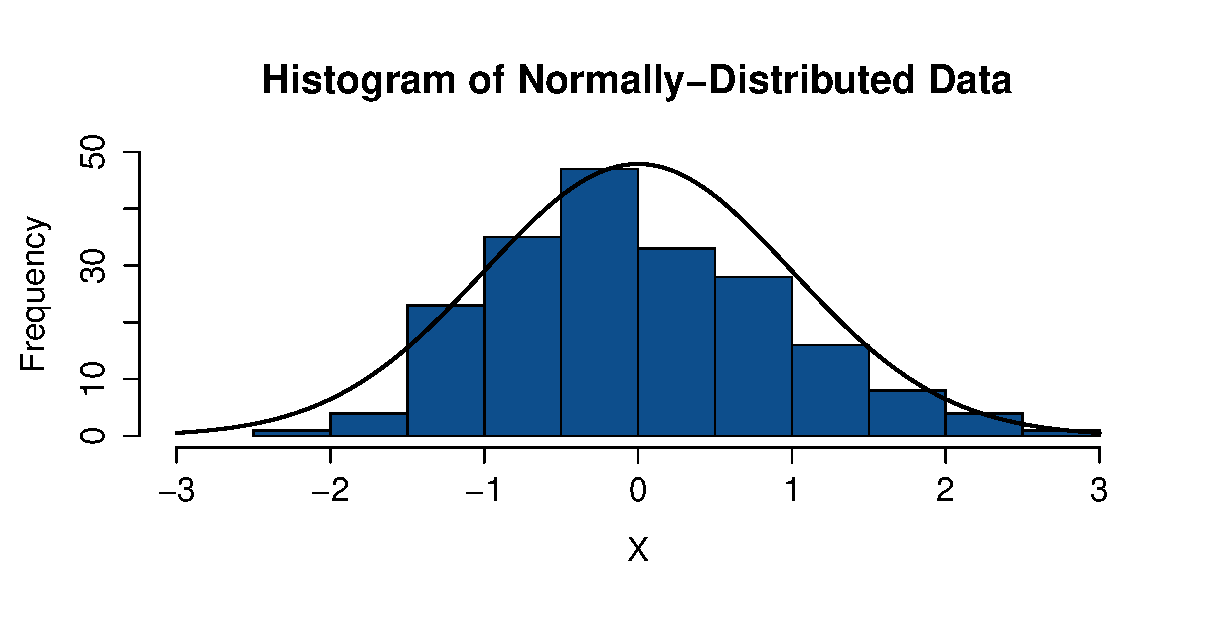
\includegraphics[width=35pc]{uncertainty01}
\caption{Histogram of approximately normal data with a slight rightward skew}
\label{fig:uncertainty01}
\end{figure}

The smooth line that you see there is the \textbf{normal distribution}; the columns represent our actual observations. As you can see, the two don't line up perfectly. Rather, our graph is stretched out to the right a bit. We call this stretching \textbf{skewness}: the idea that, rather than being perfectly symmetrical about the mean, out data are stretched out to the right or to the left. In cases where our data are stretched out to the right, we say that they are skewed right; when they are stretched to the left, we say they are skewed left.

Many times, as in this example, there isn't very much skewness and our data, even though they aren't perfect, are still fairly symmetrical. However, sometimes we will have strong outliers that really mess up that symmetry. For instance, take Figure \ref{fig:uncertainty02}.

\begin{figure}[h!]
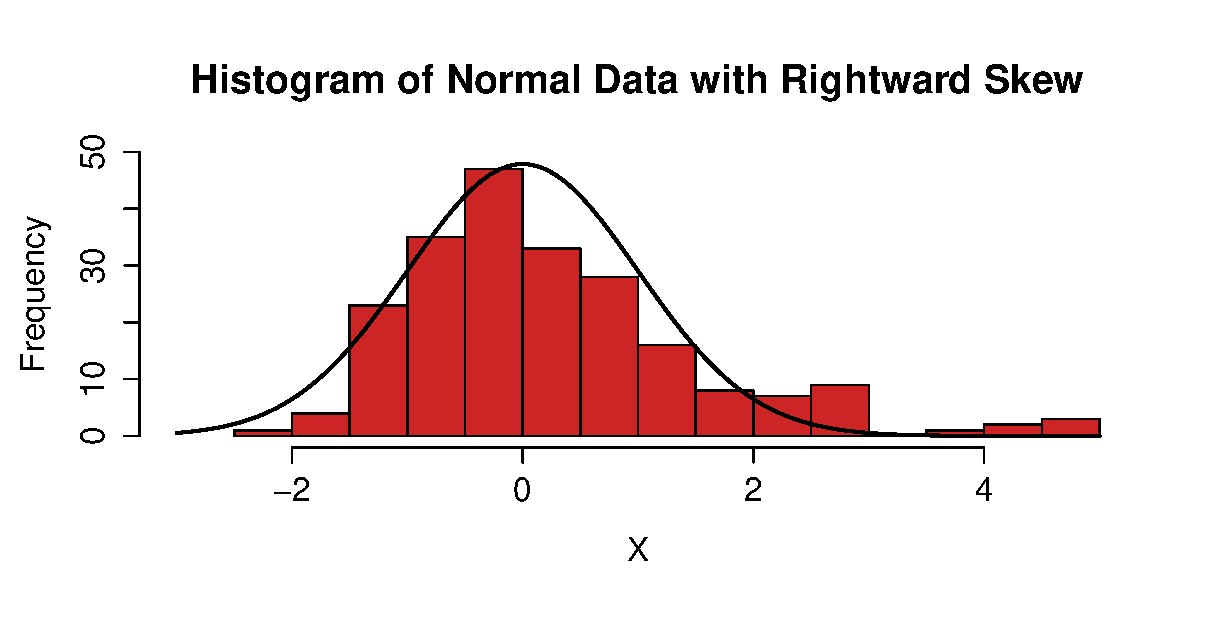
\includegraphics[width=35pc]{uncertainty02}
\caption{Histogram of data heavily skewed right}
\label{fig:uncertainty02}
\end{figure}

There, we have a strong and obvious rightward skew. Now, let's go ahead and compare the means and medians of our two datasets:

\begin{framed}
\begin{Verbatim}[samepage=TRUE]
# First we'll compare the means
> mean(data)
[1] -0.01144155
 
> mean(data2)
[1] 0.2489018
 
# And now the medians
> median(data)
[1] -0.1061751
 
> median(data2)
[1] -0.005767173
\end{Verbatim}
\end{framed}

As you can see, both the mean and the median change. However, the median changes much less than the mean does. (There's a change of 0.26 in the means versus a change of 0.10 in the medians.) In cases where you have strongly skewed data, it will often be better to describe them using the median rather than the mean: specifically, the median is what we call \textbf{resistant to outliers}. In other words, when you have a few outliers (numbers that are far away from every other data point), the median will be changed much less than the mean will.

\section{Standard Deviation}
\textbf{Standard deviation} (represented as $s$ or $\sigma$) is a measure of dispersion: that is, it tells us how far from or close to the mean our data tend to be. A data set with a small standard deviation, for instance, tells us that most of our data points are fairly close together and are all near the mean. Alternately, a large standard deviation means that our data points are much more spread out. We can visualize this using three data sets, all with mean $\mu=0$ but with different standard deviations, as in Figure \ref{fig:uncertainty03}.

\begin{figure}[htp]
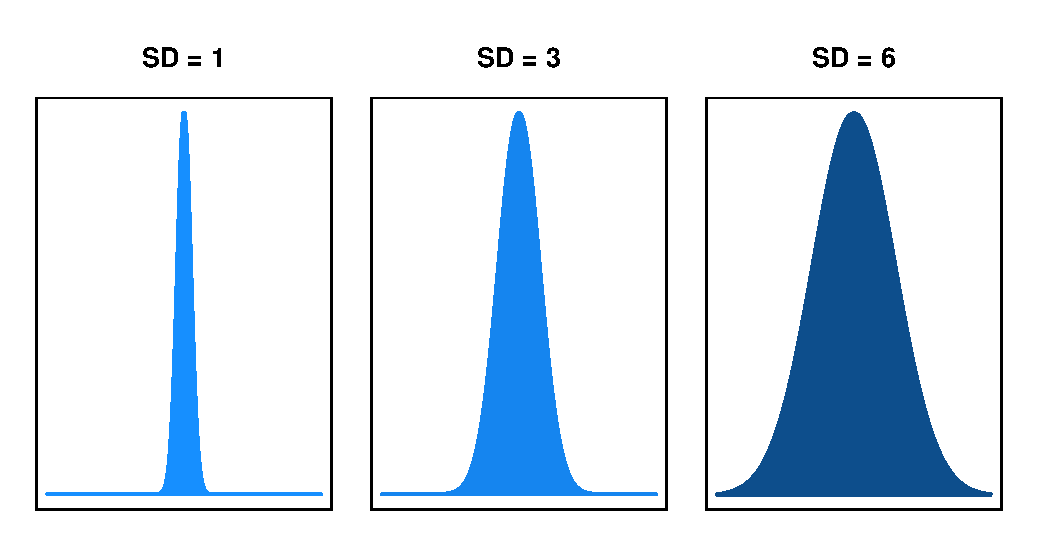
\includegraphics[width=35pc]{uncertainty03}
\caption{Three samples of data with mean \(\mu=0\) and standard deviations of 1, 3, and 6, respectively.}
\label{fig:uncertainty03}
\end{figure}

Even though each of these three sets of data has the same mean (0), it's pretty clear that there are some big differences between each of them. This is why standard deviation is important to know and report: without it, you aren't going to be getting a complete picture of what your data look like. They could all be close to the mean, as in the graph on the far left, or they could be much more spread out, as in the graph on the right.

Now, before we can use standard deviations, we have to calculate them. The formula for standard deviation looks like:

\begin{equation}
\sigma = \sqrt{
	\frac{1}{n}\sum_{i=1}^n\left(x_i-\mu\right)^2
	} \text{, where }
	\mu=\frac{1}{n}\sum_{i=1}^n(x_i)
\end{equation}

Let's unpack that: it's saying that we start by finding the mean ($ \mu $) of the data. Next, we'll go ahead and take every data point and subtract the mean from it (the $ x_i-\mu $ part of the equation). So what we're doing is basically finding out how many units away from the mean each data point is. But there's a problem: some data points might give us a negative number, others a positive number. So we'll take that difference and raise it to the second power (remember, a negative number times a negative number is always equal to a positive number). Now we just repeat that for every other data point in our sample and add them all together.

So now we have summed up all of those squared differences, right? Next, we will divide by the number ($ n $) of observations (just like when we calculated the mean) to get the \textbf{average distance from the mean}. But there's one last step before we're done: since we raised everything to the second power a couple steps ago, we have to undo that operation. To do this, we'll take the square root of everything, leaving us at last with the standard deviation.

\subsection{Variance}
In many ways, variance and standard deviation are two sides of the same coin. If you remember, standard deviation is calculated:

    \[ \sigma = \sqrt{\frac{1}{n}\sum_{i=1}^n\left(x_i-\mu\right)^2}\text{, where } \mu=\frac{1}{n}\sum_{i=1}^n(x_i) \]

Variance, then, is:

\begin{eqnarray*}
	\sigma^2 &=& \frac{1}{n}\sum_{i=1}^n\left(x_i-\mu\right)^2 \\
	&=& \left(\frac{1}{n}\sum_{i=1}^nx_i\right)-\mu^2\text{, where } \mu=\frac{1}{n}\sum_{i=1}^n(x_i)
\end{eqnarray*}

So, we can see that population variance is calculated exactly the same as is standard deviation, except we never take a square root at the end of it all. But if they're calculated so similarly and they both measure essentially the same thing, why would we use one over the other and why do we have both?

One big reason for using standard deviation instead of variance, at least in applied statistics, is that the standard deviation is in the same units as your data. (E.g., if you're looking at weights, the standard deviation is in pounds.) Variance, on the other hand, is in squared units. (So instead of pounds, you'd have a variance in pounds squared. That's less easy to interpret, isn't it?) Beyond this, standard deviation also gives us the 65-97-99.5\% rule.

This rule tells us that 65\% of all observations in a normal distribution will fall within 1 standard deviation of the mean; 97\% will fall within 2 standard deviations of the mean; and 99.5\% will fall within 3 standard deviations of the mean. We can illustrate this in Figure \ref{fig:uncertainty04}:

\begin{figure}[h!]
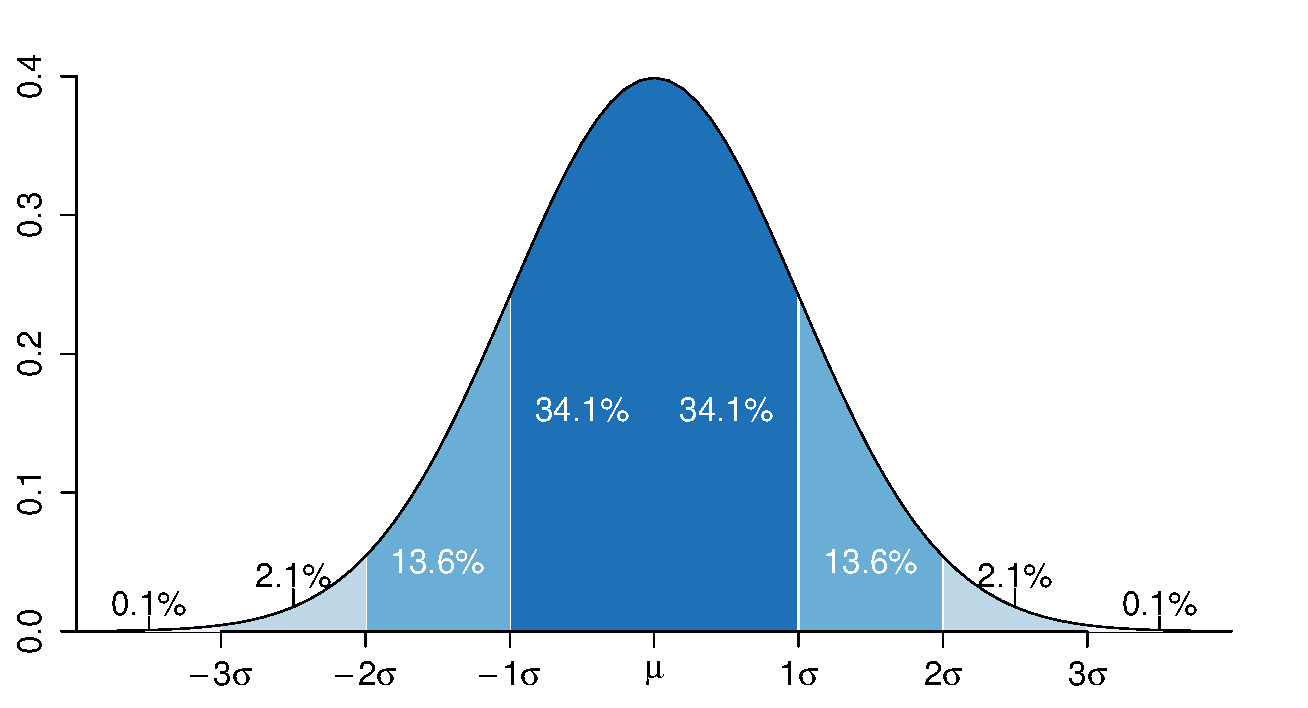
\includegraphics[width=35pc]{uncertainty04}
\caption{The 68-97-99.5\% rule states that nearly all observed data points will be within 3 standard deviations of the mean. This is often useful for flagging outliers or inappropriate distributions to fit your data to. Source: \href{http://en.wikipedia.org/wiki/Standard_deviation}{Wikipedia}}
\label{fig:uncertainty04}
\end{figure}

So, for instance, if we wanted to find what proportion of our data would be more than 1 standard deviation above the mean, we would add 13.6\%, 2.1\%, and 0.1\% to end up with 15.8\% of our data being more than 1 standard deviation above the mean.

\begin{framed}
\noindent \textbf{{\large Remember:}}

\textbf{Standard deviation} is the average distance of a data point from the mean of your data. \textbf{Variance} is the squared average distance of a data point from the mean. Standard deviation is always in the same units as your data; variance is in units\(^2\).
\end{framed}

\subsection{Interquartile Range}
The last measure of spread that we will discuss is the interquartile range. This is most commonly used when the median used rather than the mean. This number is based off of what is known as the ``5-number summary,'' defined as:

\begin{glossary}
\term{Minimum}{The smallest value in your data set}
\term{Q1}{The value in your data set that is larger than 25\% of all other values}
\term{Median}{The median value in your data set}
\term{Q3}{The value in your data set that is larger than 75\% of all other values}
\term{Maximum}{The largest value in your data set}
\term{}{}
\end{glossary}

You'll quickly recognize this information if you're familiar with boxplots (if not, we cover them below). To derive the interquartile range (IQR) from these, we simply take Q3 - Q1. From the definitions above, we know that exactly 50\% of our data points lie between these two values. Given this, the IQR can be said to be another measure of the dispersion of our data: instead of a 65-97-99.5\% rule, here we have a 50-25-25\% rule: 50\% of our observations lie within the range given by the IQR; 25\% lie above it; and 25\% lie below it. As with standard deviation, a smaller IQR indicates a tighter spread of data (i.e., more of the data points are squished together) and a larger IQR indicates more variance of the data.

Finally, the IQR is often used to identify outliers in a data set. To do this, we will usually find our upper and lower cutoffs by:

\begin{eqnarray*}
    \text{Upper} &=& Q3+1.5\cdot IQR \\
    \text{Lower} &=& Q1-1.5\cdot IQR
\end{eqnarray*}

That is, any data point more than 1.5 times the IQR above Q3 or more than 1.5 times the IQR below Q1 can be considered suspect and possibly an outlier. Important to note, however, is that this isn't a hard-and-fast rule: there is no real reason that we use 1.5 times the IQR as a cutoff. (Actually, the statistician who came up with this measure chose 1.5 times because 1 seemed too small and 2 seemed too large.)

\section{Sampling Distributions}

\subsection{Central Limit Theorem and Sampling Distributions}
Does the central limit theorem ring any bells? Probably not. But it's still probably something that you've heard of before. Specifically, you may have heard of it in the context of \textbf{regression to the mean}. This is the idea that (let's use height as an example) if you randomly choose one adult male in the U.S., his height could very easily be 7'3". That's obviously a lot taller than most people. But the next person you choose will probably have a height less than the first guy's. And if you keep choosing more and more people and measuring their heights, pretty soon, the average height of everyone you chose will be pretty darned close to the actual national average height for adult males. More generally, the idea is that every now and then there will always be extreme scores. But every time you get one of those strong outliers, the next observation is almost certainly going to be less extreme and it is going to pull things back down to the population average.

The \textbf{central limit theorem} is sort of similar: it states that the distribution of an average tends to be normal, even if the population is not itself normal.

Make sense? Maybe not (that's okay!), so let's break it down a bit. Whenever we're talking about a distribution of averages, we call that a \textbf{sampling distribution}. To continue with our height example from above, let's say that we randomly choose 25 guys and measure their heights. Then we choose another 25 guys and measure their heights. Then we choose another 25 guys and measure their heights. Assuming that the mean male adult height is 5'8" with a 4" standard deviation (we have to represent that with decimals in R, so it becomes a mean of 5.67 feet and a standard deviation of 0.33 feet), our three samples might look like Figure \ref{fig:uncertainty05}.

\begin{figure}[h!]
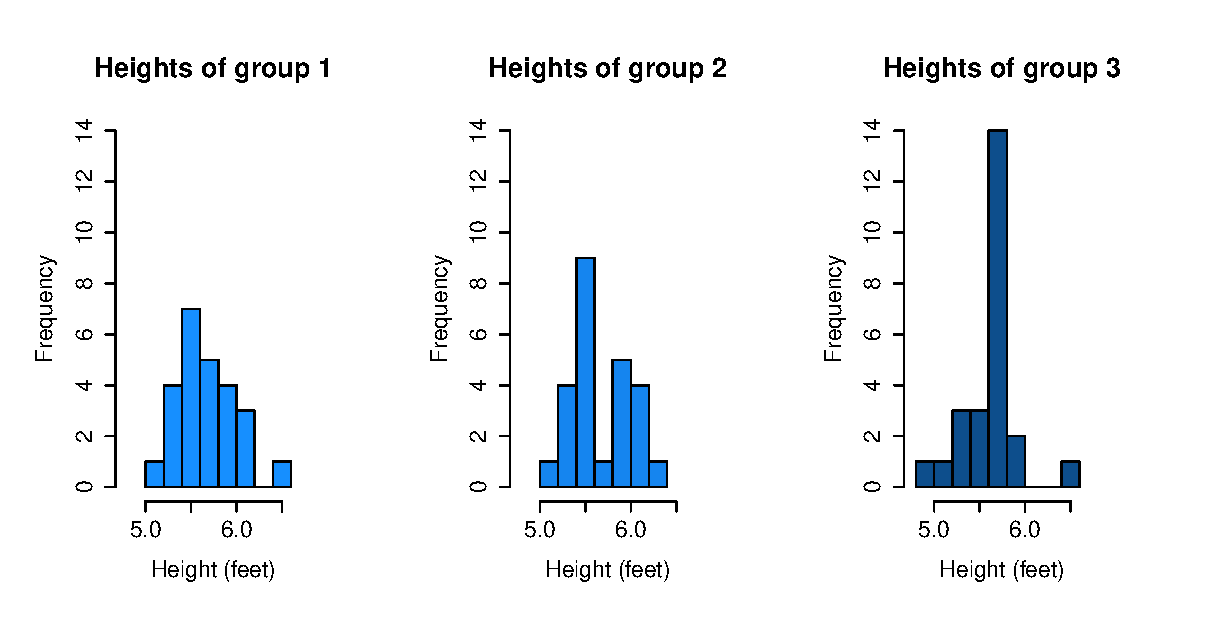
\includegraphics[width=35pc]{uncertainty05}
\caption{Heights of three randomly-selected groups of men}
\label{fig:uncertainty05}
\end{figure}

We can see that there's a lot of variation among our three groups, right? And groups 2 and 3 don't really look all that normal. But, let's say that we take the average male height of each of our three samples. Now, let's repeat that with another 497 batches of 25 men each. If we make a histogram of the average height from each of those 500 groups, it will look like Figure \ref{fig:uncertainty06}.

\begin{figure}[h!]
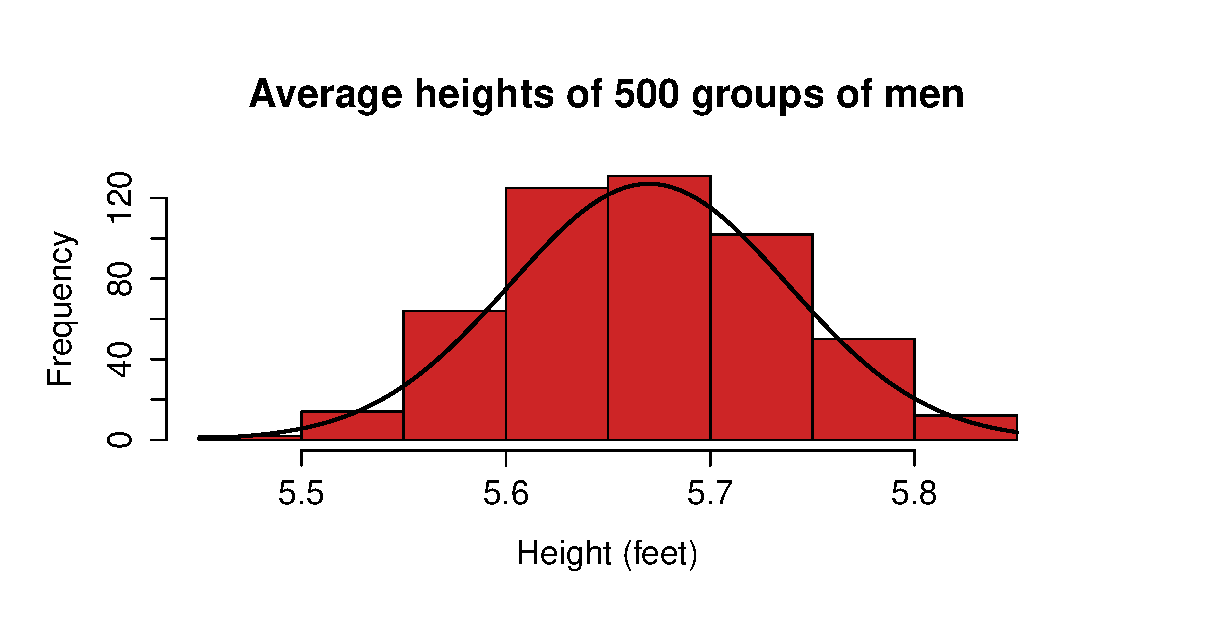
\includegraphics[width=35pc]{uncertainty06}
\caption{Average height of 500 groups of randomly selected men}
\label{fig:uncertainty06}
\end{figure}

All of a sudden, we have a normal distribution with a mean height of 5.67 feet (or 5'8") and a standard deviation of 0.068 feet (or 0.81 inches). We see that the mean of our sampling distribution is exactly equal to the mean of our population: that's the central limit theorem in action.

\subsection{Standard Error}

You might have noticed that the standard deviation of the sampling distribution above was much smaller than the standard deviation of the actual population (0.81 inches versus 4 inches). This arises because we're looking at the variation of a set of means (which themselves are the average value of a larger set of data): these will always vary less than the individual data points that we sample from. And actually, when we're talking about the variation of sample means, instead of standard deviation, we will want to use what's called the \textbf{standard error}, a specific term referring to the standard deviation of a sampling distribution. This will always be smaller than the standard deviation of the population and can be estimated by:

\begin{equation}
\text{SE}_{\bar{x}}= \frac{s}{\sqrt{n}}
\end{equation}

Here, \(s\)  is the sample standard deviation (here, 0.81 inches) and \(n\)  is the number of observations (that is, the number of samples---here, 500). As you can see, the standard error is always going to be smaller than the population's actual standard deviation. In short, the \textbf{standard error} is a measure of how far a sample mean is likely to be from the population mean; the \textbf{standard deviation} is a measure of how far an individual observation is likely to be from the sample mean.

\section{Visualizing Data}

\subsection{Histograms}
A \textbf{histogram} displays the number of observations that fall within a given range. For instance, in the height examples above, we would count the number of men in our sample between 5 feet and 5.2 feet and display them all in one column. Then we'd do the same for 5.2 to 5.4 feet, for 5.4 to 5.6 feet, and so on. This gives us something like:

\includegraphics[width=35pc]{uncertainty07}

\subsection{Kernel Density Plots}
A kernel density plot is similar to a histogram in that it shows us about what proportion of our sample is likely to be at any certain value. The big difference between kernel density plots and histograms is that density plots are continuous: whereas histograms take all of your data and lump them together in ranges, a density plot displays these data continuously. For instance, taking the same data that we used in our histogram example:

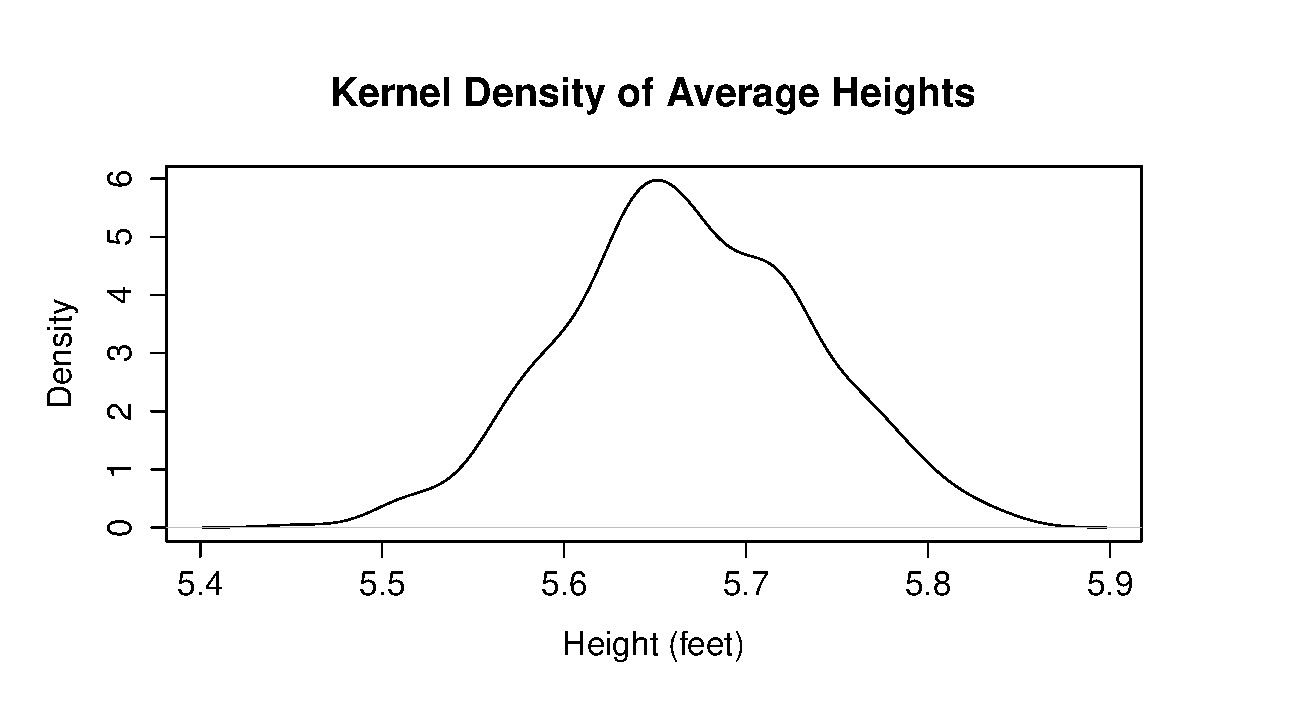
\includegraphics[width=35pc]{uncertainty08}

Comparing the two graphs, they tell about the same story. However, the kernel density plot isn't subject to issues of binning. Specifically, when using histograms, the width of the bins that you use (or the range of each column) can drastically impact your interpretation of the data. For instance, if we increase the number of bins, we get something like:

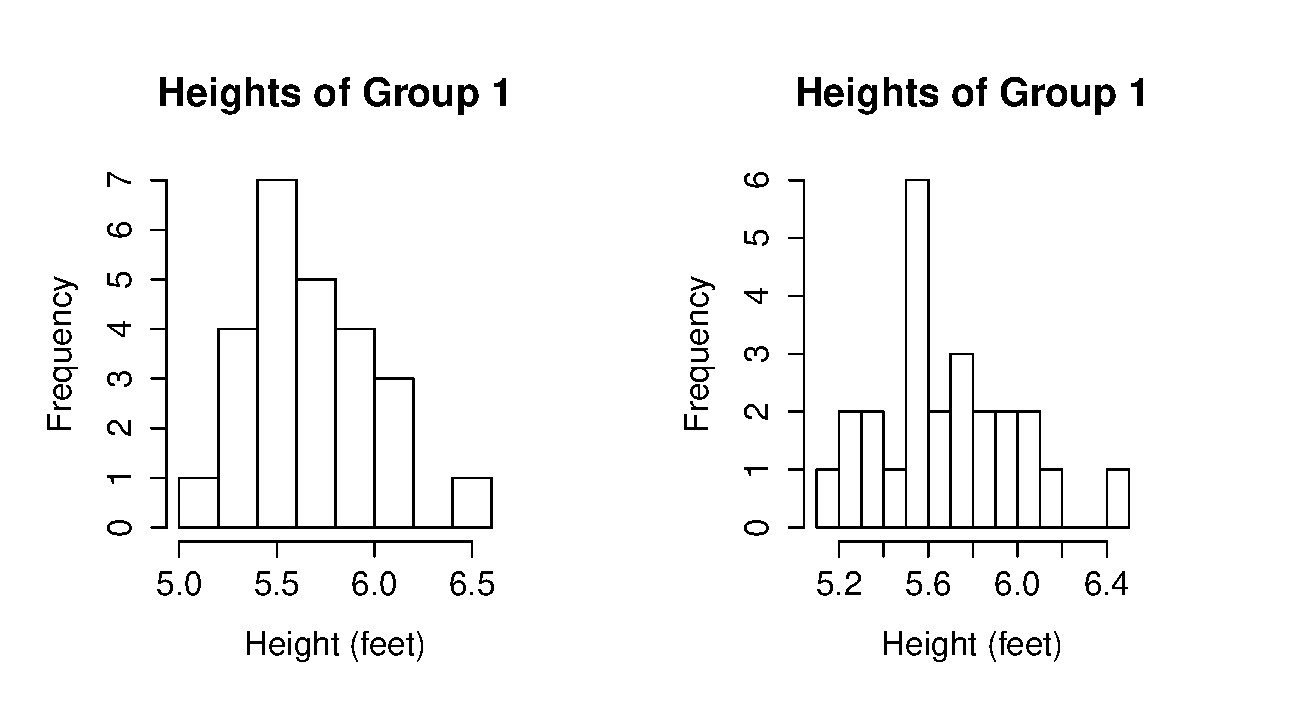
\includegraphics[width=35pc]{uncertainty09}

As the range of each bin varies, we can go from a nice-looking normal distribution to a much worse looking non-normal distribution. But with a kernel density plot, you remove those issues in interpretation:

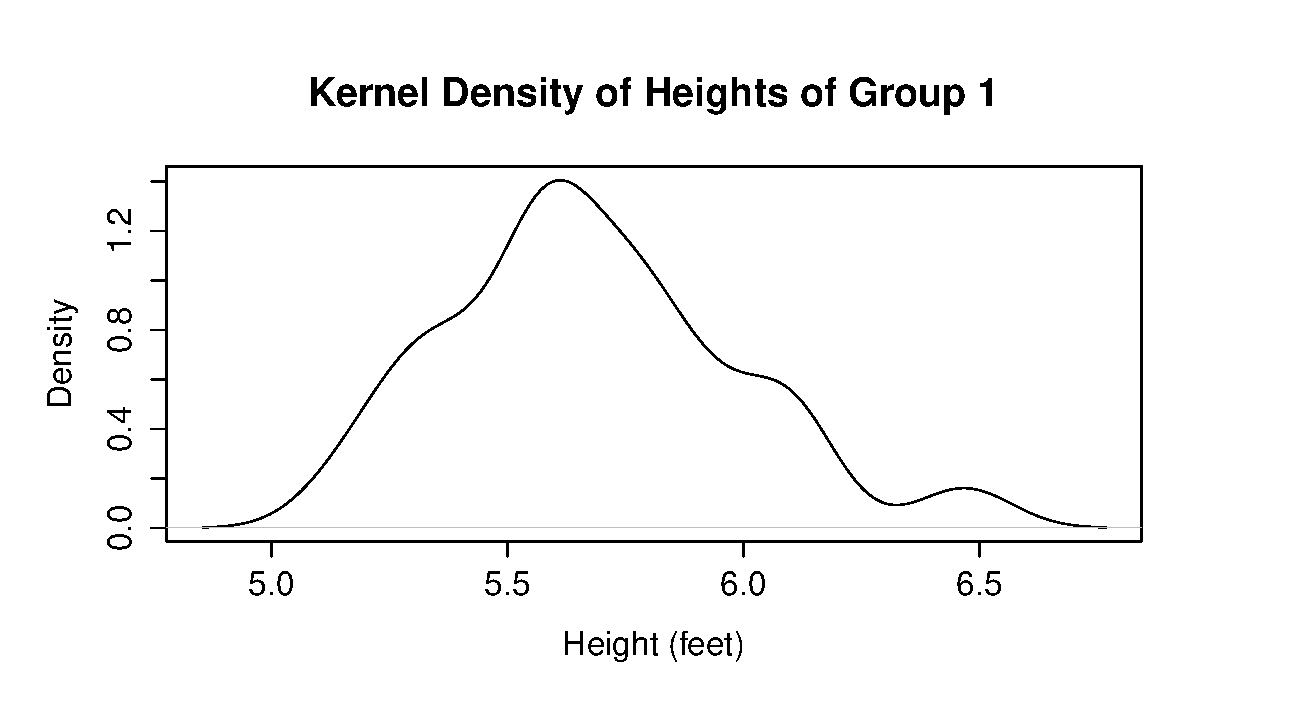
\includegraphics[width=35pc]{uncertainty10}

As we can see, in reality, it actually is a roughly normal distribution with some funky skewness over to the right.

\subsection{Boxplots}

As discussed previously, boxplots are good to use when you're working with the median, interquartile range, and 5-number summary. These take that 5-number summary and present the data visually:

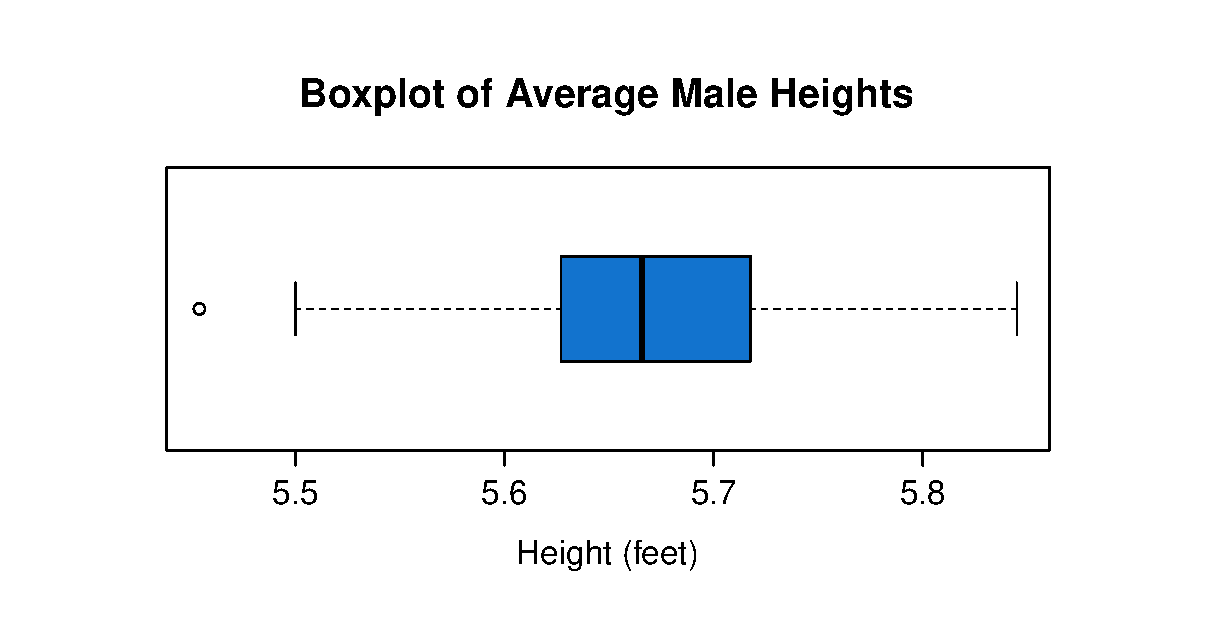
\includegraphics[width=35pc]{uncertainty11}

Here, the line on the far left is the minimum value, the left edge of the box is Q1, the line bisecting the box is the median, the right edge of the box is Q3, and the line to the far right is the maximum value. Any circles indicate the presence of outliers based on the IQR.
\section{Exercises}

\prob In R, execute the following code:
\begin{framed}
\begin{Verbatim}[samepage=TRUE]
set.seed(0)
height1 <- rnorm(25, 5.6667, 1/3)
 
avgHeight <- NULL
 
for(i in 1:500) {
  height <- rnorm(25, 5.6667, 1/3)
  avgHeight <- rbind(avgHeight, mean(height))
}
\end{Verbatim}
\end{framed}

\prob What are the mean and median values of \verb|height1| and \verb|avgHeight|? What are their standard deviations?

\prob What would we expect the standard error of \verb|avgHeight| to be if we had 500 samples and a population standard deviation of 0.33 feet?

\prob Prepare a histogram of \verb|height1| and \verb|avgHeight|. Do they differ? Does either look problematic? (E.g., departures from normality)

\prob Make a kernel density plot of \verb|height1|. Does it differ from the histogram? Which gives a better picture of the data?

\prob Make a boxplot of \verb|avgHeight|. Are there any outliers present?

\section{Additonal Resources}
\begin{enumerate}
	\item \href{https://github.com/faulconbridge/appliedStats/blob/master/LaTeX/part01/RScripts/uncertainty.R}{R script} containing all commands used in examples throughout this chapter
	\item \href{https://github.com/faulconbridge/appliedStats/blob/master/LaTeX/part01/answers/uncertainty.md}{Answer key} for the chapter's exercises
\end{enumerate}
	\include{part01/researchDesign}
	%!TEX root=../book.tex

\chapter{Introduction to Statistical Inference}

\section{What Is Statistical Inference}

\subsection{Its Purpose}
Statistical inference provides formal methods for drawing conclusions about a population from sample data. That is, statistical inference refers to the whole suite of quantitative tools that we have developed to test data-driven hypotheses, accounting for random variation in those data. These are the tools that we will spend the remainder of the book discussing in some degree of depth.

We have developed these statistical models to make predictions about populations and to draw conclusions about differences between populations. These lie in contrast to both descriptive statistics and purely qualitative methods. More correctly, we might say that all three lie on a spectrum with qualitative measures being employed to provide a very general overview of a topic without seeking to address substantive differences among populations or to predict future trends. Oftentimes this type of research is used to inform later quantitative studies by providing new directions for research based on participant opinions, beliefs, and feedback.

Squarely in the middle lie descriptive statistics: these provide a descriptive overview of a set of data; however, they are not (in and of themselves) able to predict trends or quantify difference. It is only when they are applied in the context of statistical models that they can be used to reach decisive conclusions from and about our data.

\subsection{Hypotheses for Means}
In statistical inference, we often form hypotheses about our data. These will generally take the form of a null and alternative hypothesis. Alternative hypotheses may be one- or two-sided. The null hypothesis (abbreviated \(H_0\); pronounced ``H-null'') always predicts that there is no difference between our control and treatment groups (i.e., \(H_0: \mu=\mu_0\) where \(\mu\) is the mean of our treatment group and \(\mu_0\) is the mean of the control group). Predictably, the alternative hypothesis (\(H_A\); pronounced ``H-A'') predicts that a difference in our two groups exists. If one-sided, it predicts a direction of the difference (e.g., \(H_A: \mu > \mu_0\); two-sided hypotheses predict only that a difference exists, but are agnostic as to the direction of that difference (\(H_A: \mu \neq \mu_0\)).

We also operate with the understanding that is easier to prove something as false than as true. Given this, the null hypothesis is always presumed true until sufficient evidence is found supporting the alternative hypothesis. Importantly, though, we do not ever formally accept the null hypothesis: we may only fail to reject it. (Recall again that most inferential statistics seek to disprove a hypothesis rather than prove it.) In this way, we may fail to reject the null hypothesis, but never accept it. (However, we may accept the alternative hypothesis. By disproving the null, we are demonstrating that its converse must, by that fact, be true.)

\subsection{Test Statistics and Statistical Significance}

\subsubsection{Standardized Test Statistics}
Whenever we perform a statistical test, we are usually given two important pieces of data: a test statistic and a \textit{p}-value. Standardized test statistics can take a number of different forms (z-, t-, and F-statistics are three of the more common) and each has a slightly different interpretation. However, speaking generally, every \textbf{test statistic} is a single, quantified measure for assessing patterns in the data that distinguish between the null and alternative hypotheses.

\subsubsection{Degrees of Freedom}

Degrees of freedom is one of those concepts that (at least in the social sciences) is mentioned briefly and then promptly forgotten for the rest of your career. And that's darned unfortunate, because degrees of freedom is actually an important concept and fairly nuanced to explain to a non-mathematical audience (and frankly deserving a better treatment than we give it here).

A basic definition of the concept is the ``number of observations minus the number of necessary relations among these observations'' (via \href{http://dx.doi.org/10.1037%2Fh0054588}{Walker, H.}. In other words it's the total number of observations in your sample minus the number of parameters being estimated.

The thinking behind this goes that your sample data can be used to estimate one of two things: the variance of the population or a parameter (e.g., a piece of data can be used to estimate the population mean or standard deviation, but not both). Now, generally, each parameter being estimated takes up only one degree of freedom with the rest left to estimate variance. That doesn't always hold true, such as when using Welch's \textit{t}-test, but it's close enough for our purposes.

Again, we can't emphasize enough how much better an explanation this concept deserves and we strongly recommend that you take an afternoon to read up on it. Gerard Dallal's \href{http://www.jerrydallal.com/LHSP/dof.htm}{Degrees of Freedom} might be a good place to start!

\subsubsection{Probability Values}
Accompanying the test statistic is the \textbf{\textit{p}-value}. Universally, this measure has a single interpretation: it is the probability (from 0 to 1, inclusive) that the differences observed in the data arise due to chance and natural random variation. As such, smaller \textit{p}-values indicate that there is a smaller probability of the differences seen being due to chance. Many disciplines impose a ``5\% rule'' on this statistic: that is, they consider any \textit{p}-value less than 0.05 (or 5\%) as being statistically significant.

We use the term \textbf{statistically significant} to indicate that we are reasonably confident that the differences observed in the data are in fact due to an experimental manipulation or some actual difference between the groups we're looking at. There is no specific reason for using a threshold of 5\%---and indeed sometimes a 1\% or 0.1\% cutoff will be used instead---; however, this is the most commonly-agreed-upon threshold for describing a test as significant.

Important to keep in mind (really! This is important) is that a \textit{p}-value is \textbf{not} a posterior probability of the truth of the null hypothesis; rather, it \textbf{is} a probability conditional on the null. What does that mean? Well, it's the difference between saying ``Given our data, there is a 5\% chance that the null hypothesis is true'' and ``Given that the null hypothesis were true, there is only a 5\% chance that our data would look the way they do.'' See the difference there? (Not to belabor the grammar, but the second statement is careful to use the subjunctive, the idea being ``if we assume this to be true although it might not actually be''.)

One further consideration when performing statistical tests is that statistical significance is not the same as practical significance. Two sets of data can easily be statistically significant without being practically significant. As an example, consider patient scores on a depression questionnaire: groups from two different clinics may have significantly different scores, but if the mean scores still classify both groups as chronically depressed, a couple-point difference doesn't make a particularly meaningful impact on either group's treatment. As such, it may often be important to distinguish between what differences are statistically significant and what differences have a practical, meaningful significance.

All told, \textit{p}-values are picky and noisy statistics that are hard to compare across studies. If you're interested in reading more about cautions in their interpretation, try \href{http://www.stat.columbia.edu/~gelman/research/published/pvalues3.pdf}{this article by Gelman} for starters.

\subsubsection{Confidence Intervals}
Statistical tests will also typically provide a \textbf{confidence interval} for the true parameter value. That is, this measure gives a range that, with some percent confidence, should contain the ``true'' value that the researcher is trying to measure. For example, if a researcher wished to know if there was a difference in average heights of boys and girls at age 8, a 95\% CI from 0.3 -- 0.9 would indicate that there was a 95\% chance that the true mean difference in height (i.e., if we measured the height of every 8-year-old boy and girl in the world) was between 0.3 feet (or 4 inches) and 0.9 feet (or 10.8 inches). Given that this confidence interval doesn't contain 0 (which would indicate that there is no difference in heights), we can likely assume that there does exist a difference in mean height between our two populations.

\section{Some Considerations about Statistical Inference}

\subsection{Conditions for Inference}
For our conclusions about statistical tests to be valid, there are always assumptions that need to be met about the data. These assumptions differ from test to test; however, they generally require a random sample (or at least a representative sample) of the population to have been selected. Many times the test will also require that the data not be significantly skewed by outliers or that samples have equivalent variance. In any case, with each test presented we will clearly outline the assumptions that must be met as well as those that should be met but that can be violated without necessarily invalidating the test.

\subsection{Cautions about Significance Tests}
\subsubsection{How Small a \textit{p}-value?}
As mentioned above, the magnitude of a \textit{p}-value needed for a result to be called ``significant'' is arbitrary: 5\% simply happens to be what is widely agreed upon. However, this still means that 1 out of every 20 experiments will tell the researcher that a significant difference exists when there actually isn't one. If we use a 1\% threshold, that drops to 1 in every 100 trials. Still more stringent is 1 in 1000 trials, or a 0.1\% cutoff. But how small or large a \textit{p}-value do we really need to convince us of an effect?

Many times, a much smaller \textit{p}-value will be needed to refute a well-established theory. However, if you are exploring a new program of research, larger \textit{p}-values may be fine if they are simply exploratory analyses that will be used to indicate potential avenues for further research.

\subsubsection{The Danger of Multiple Tests}
When performing statistical analyses, if a researcher analyses the data enough different ways, eventually he or she will obtain statistically significant results. By sheer chance, this is bound to at some point happen. However, one significant result among 20 non-significant results does not constitute strong evidence against a null hypothesis. Rather, this is a process known as \textit{p}-hacking: the practice of waiting until a researcher finds an analysis that will produce a favorable result and then reporting that test as definitive evidence in favor of his or her hypothesis.

\subsubsection{Type I and II Errors}
Lastly is the issue of errors regarding your conclusion about a statistical test. A \textbf{Type I Error} is equivalent to a false positive. This occurs when a researcher achieves a significant \textit{p}-value (i.e., $p\text{-value}<0.05$) and rejects the null hypothesis when there is actually no evidence for doing so. If you recall from above, $p\text{-value}=0.05$ means that every 1 in 20 experiments, the researcher will have a significant \textit{p}-value when there actually isn't any difference in the populations. This is a ``fluke'' that is usually caused by sampling bias or some similar error. Regardless, it ends up that the researcher rejects the null hypothesis when he or she shouldn't have.

Conversely, a \textbf{Type II Error} is a false negative, occurring when a researcher fails to reject a null hypothesis despite there actually being a significant difference between the populations being studied. This may be caused by a small sample size, small effect size or power, etc. This distinction can alternately be represented:

\begin{center}
\begin{tabular}{|r c c|}
\hline
& $H_0$ is true & $H_0$ is false \\
 Reject $H_0$ & Type I Error & Correct\\
Fail to reject $H_0$ & Correct & Type II Error\\
\hline
\end{tabular}
\end{center}

The probability of a test making a Type I error is denoted $\alpha$; the probability of making a Type II error, $\beta$.

\section{Recap: The Components of a Statistical Test}

To recap, there are 6 main components to any statistical test and write-up: the research question, hypotheses, fundamental and standardized test statistics, the \textit{p}-value, and the overall conclusion. As an example, let's say that we are interested in determining whether there is a significant difference in the average heights of 12-year-old boys and girls. Those six steps would look something like:

\begin{center}
\begin{tabular}{r l}
Item & Example \\
\hline
Research Question & Is there a difference in the average heights of boys and girls at 12 years old?\\
Hypotheses & \parbox[t]{25pc}{\(H_0:\) boy height = girl height\\\(H_A:\) boy height \(\neq\) girl height}\\
Fundamental Statistics & \parbox[t]{25pc}{Average boy height = 4'10'' \\ Average girl height = 4'11''}\\
Standardized Statistics & This is the t-, z-, F-, etc. statistic that a statistical test will give you.\\
\textit{p}-value & The statistical test will also give you a \textit{p}-value that is between 0 and 1.\\
Conclusion & \parbox[t]{25pc}{If the \textit{p}-value is less than $p\text{-value}=0.05$, most disciplines will consider that significant evidence against the null hypothesis (\(H_0\)), meaning that we can reject it and accept the alternate hypothesis. In this case, that would mean that there \textbf{is} a significant difference between the average heights of girls and boys at age 12.}
\end{tabular}
\end{center}

Of course, working with real data the second half of the table would look a bit different; however, it would keep that general form. If you're still a little fuzzy on any of the specific elements of a statistical write-up, that's fine: we'll go over it all again each time we present a case study alongside a new statistical test.

	
	\part{Comparisons Among Multiple Samples}
	%!TEX root=../book.tex

\chapter{\textit{t}-Tools}

\section{Overview of \textit{t}-Tools}

\subsection{One-Sample \textit{t}-tools}

The one-sample \textit{t}-test is one of the simplest entry points to inferential statistics there is. Simply put, it seeks to determine if the average value of a set of data differs significantly from some theoretical quantity. Say, for instance, we are working in a lumber mill and it looks like a shipment of Douglas fir trees is a bit smaller than usual. We know that a typical Douglas fir from this region is about 225 feet tall and has a radius of 7.5 feet, giving us a total volume of about $39000$ cubic feet.

So we take the measurements for each of the trees in this shipment and find that the average volume is $36500$ cubic feet with a standard deviation around $\sigma = 2000$ cubic feet. Do we have sufficient proof that these trees are actually smaller than our typical shipment?

Well, unfortunately, the human brain isn't great at intuitively figuring out if differences like that are meaningful or within the expected margin of error: that's where inferential statistics come into play. So let's first state our hypotheses as:
\begin{eqnarray*}
H_0:& \bar{x} = \mu\\
H_A:& \bar{x} \neq \mu
\end{eqnarray*}
where $\bar{x}$ is the mean volume of our shipment of trees and $\mu$ is the mean volume of adult Douglas firs. Now, we can conduct our statistical test.

A \textit{t}-test, speaking generally, takes the form:
\begin{equation}
t = \frac{\text{Estimate}-\text{Parameter}}{SE(\text{Estimate})}
\end{equation}
The specifics of what you plug in for the estimate and the parameter will vary a bit depending on which type of \textit{t}-test you use; however, they all are based off of this.

In our case, the one-sample \textit{t}-test will look like:
\begin{equation}
t=\frac{\bar{x}-\mu}{se_x}
\end{equation}
where each of the variables is what we defined in our hypotheses above. Plugging in our data we get:
\begin{eqnarray*}
t(124)&=&\frac{36500-39000}{2000/\sqrt{125}} \\
&=& -13.98
\end{eqnarray*}
Although we have our standardized \textit{t}-statistic, we still don't know if it reaches a level of significance or not. historically, we would have to go to a table of \textit{p}-values and look up the one that was closest to our \textit{t}-statistic given the degrees of freedom (here, 124, or $n-1$). Thankfully, we now have software that is able to compute this value for us much more precisely and quickly. In this case, we end up with a \textit{p}-value $< 0.001$, showing that the result is highly significant.

Moreover, we can infer the direction of this difference. Remember that the \textit{t}-statistic is computed by subtracting our estimated mean from our population mean: given this, a negative \textit{t}-statistic means that the sample mean is less than the population mean whereas a positive \textit{t}-statistic shows that our sample mean is greater than that of the population.

So, we can ultimately conclude that this shipment of Douglas firs is statistically significantly below the average size of a shipment, given $t(124)=-13.98$ with a $p\text{-value} < 0.001$. We can summarize this difference in Figure \ref{fig:t01}.

\begin{figure}[h]
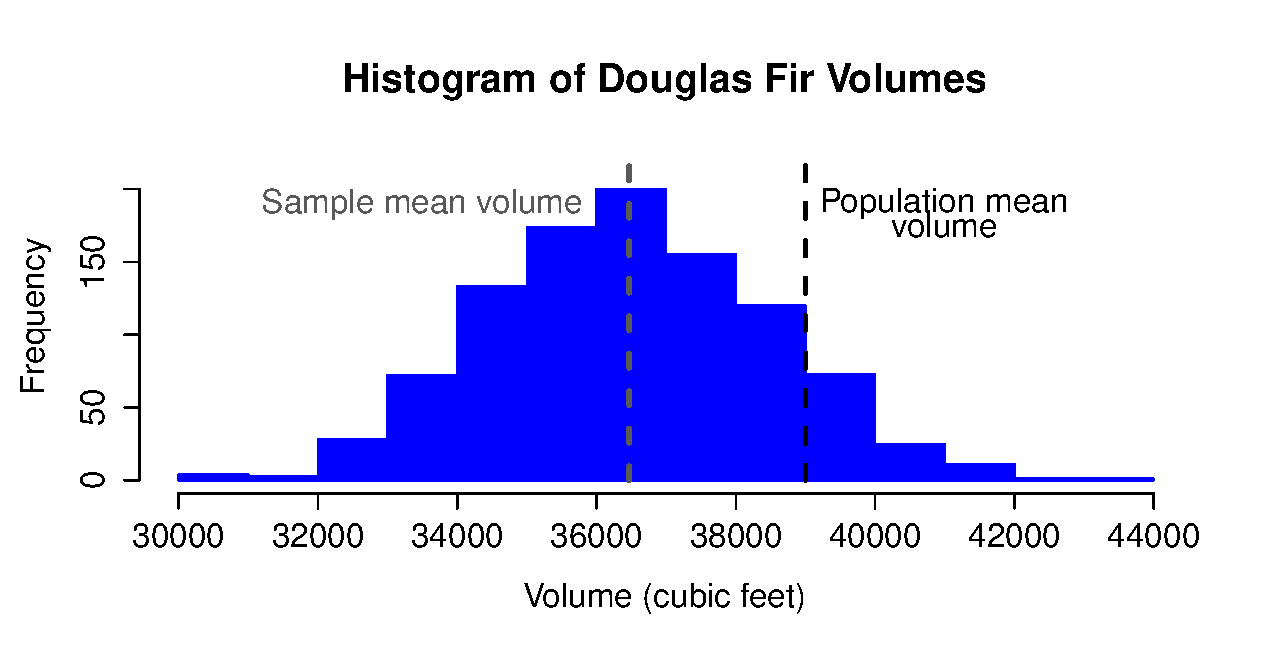
\includegraphics[width=35pc]{t01}
\label{fig:t01}
\caption{Histogram of the volumes of a shipment of Douglas firs with mean volume $36500$ cubic feet and standard deviation $\sigma = 2000$ cubic feet. A one-sample \textit{t}-test shows that this shipment of firs is significantly smaller than the typical shipment (mean $39000$ cubic feet), $t=-13.98$, $p\text{-value}<0.001$.}
\end{figure}

\subsection{Paired-Samples \textit{t}-Tools}

So now that we're familiar with a one-sample \textit{t}-test, the next two tests in the suite become really easy to understand. In a one-sample \textit{t}-test, we're testing one sample of data against a mean that we already know. I

\begin{figure}[h]
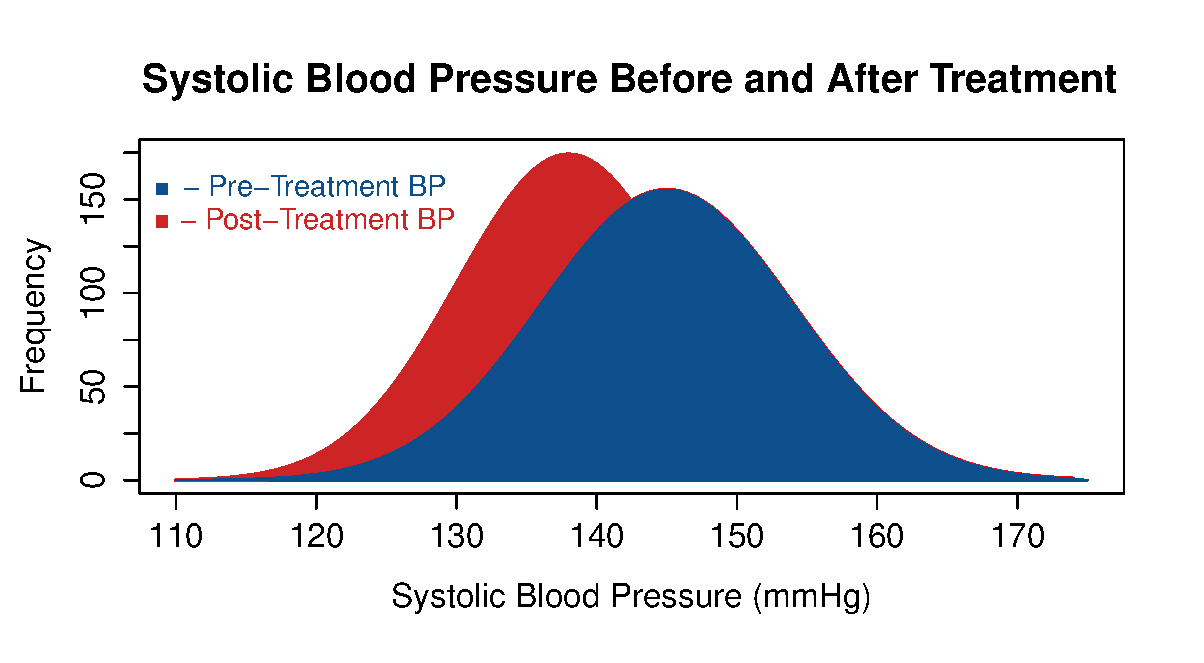
\includegraphics[width=35pc]{t02}
\label{fig:t02}
\caption{The distributions of two shipments of logs from two different logging sites.}
\end{figure}

\subsection{Independent-Samples \textit{t}-Tools}

\section{Cautions and Considerations}

\subsection{Assumptions}

\subsection{Equality of Variances}

\subsection{Robustness of \textit{t}-Tools}

\subsection{Resistance to Outliers}

\section{Implementation in R}

\section{Case Study: [STUDY]}

\section{Exercises}

\section{Additional Resources}

	%!TEX root=../book.tex

\chapter{Alternatives to $t$-Tools}

\section{Overview of Nonparametric Tools for Two Samples}

\section{Cautions and Considerations}

\section{Implementation in R}

\section{Case Study: [STUDY]}

\section{Exercises}

\section{Additional Resources}

	%!TEX root=../book.tex

\chapter{One-Way ANOVA}

\section{Overview of One-Way ANOVAs}

To understand ANOVAs, let's think back once more to \textit{t}-tests. There, we're looking to determine whether there is a difference between the means of two samples of data. But that if we want to look at more than two groups? 

Well, using what we've learned up to now, we're stuck: there's nothing more we can do. But of course that's not \textit{really} the case, is it? Otherwise we wouldn't be writing this chapter!

The idea with a one-way ANOVA (\textbf{AN}alysis \textbf{O}f \textbf{VA}riance) is that we have a variable of interest, but three or more levels of our grouping variable. For instance, we might be looking at student test scores as a function of classroom type: regular, honors, AP (advanced placement), or IB (international baccalaureate). That's way beyond the scope of any \textit{t}-test that we've come across. Thankfully, though, the ANOVA is happy to step in to fill the gap.

Before we can actually run the test, however, there is some background information that we need to understand first.

\subsection{Fixed and Random Effects}

For starters, we should be familiar with fixed, random, and mixed effects models. Broadly speaking, these refer to how the treatment factors are defined within the context of the experiment.

One caveat before we get started, though: there is no single agreed-upon definition for fixed and random effects. Rather, the precise definition is going to depend on the exact context of your experiment and your program of research. For a quick overview of these different definitions (or at least a spattering of them), check out \href{http://andrewgelman.com/2005/01/25/why_i_dont_use/}{Andrew Gelman's write-up, linked here}.

\subsubsection{Fixed Effects}

In a fixed-effects model, there is a basic assumption that the individual-specific effect is correlated with the independent variable(s). The idea here is that person-to-person, there is little variance beyond that caused by the treatment effect.

\subsubsection{Random Effects}

Random effects models assume that there is some inherent amount of individual variance not accounted for by the treatment. So if we were talking about a regression equation with a random intercept $a_i$ and fixed slope $b$, each individual would have his or hew own regression line, parallel to every other individual but with a differing intercept (cf. Figure \ref{fig:anova01}).

\begin{figure}[h]
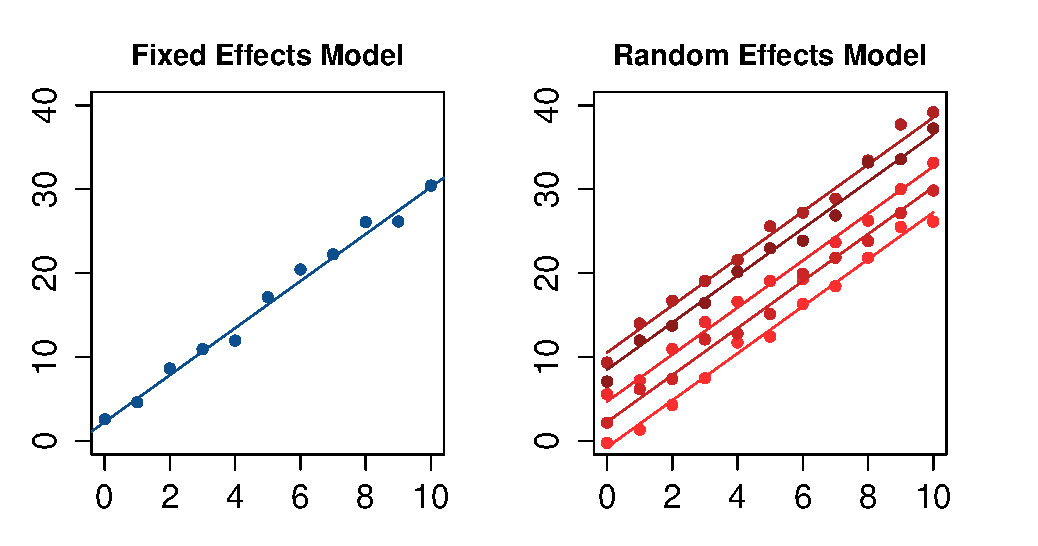
\includegraphics[width=35pc]{anova01}
\caption{A regression equation assuming fixed-effects factors for all individuals (left) and a random-effects intercept for 5 individuals (right).}
\label{fig:anova01}
\end{figure}

\subsection{Sum of Squares}

Residual, treatment, and total sums of squares are discussed more fully in our chapter on simple linear regression. The basic idea here is that there are two big sources of error: the treatment and the residual. Every time we have an experiment and are taking measurements, there is going to be some amount of background noise inherent in that: the point of statistical modeling is to reduce the amount of noise that we are unable to explain.

As such, there is noise from the treatment (individuals responding differently to the stimuli) and noise from the residual (those random fluctuations that our model is unable to explain). These combine to form a total measure of the error. In the context of an ANOVA, the residual error (termed the residual sum of squares) is equivalent to the variance within each group; the treatment sum of squares equivalent to the variance between groups. Take for instance Figures \ref{fig:anova02} and \ref{fig:anova03}.

\begin{figure}[h]
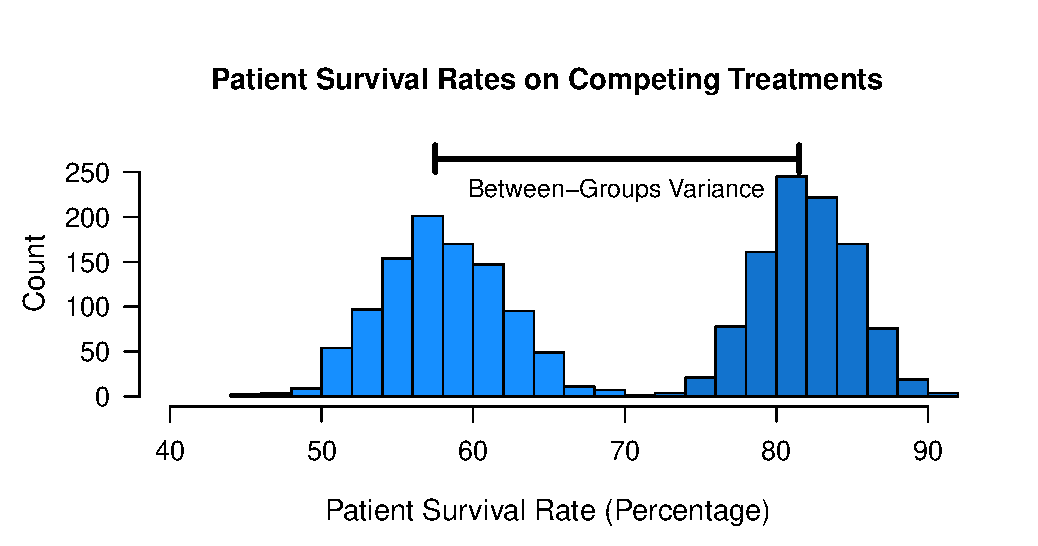
\includegraphics[width=35pc]{anova02}
\label{fig:anova02}
\caption{Patient survival rates using two competing treatment regimens. Here, between-groups variance is illustrated, showing the distance between the means of the two treatment groups.}
\end{figure}

In Figure \ref{fig:anova02}, we are looking at the difference in locations of the two treatment groups relative to one another. A greater distance between the two treatment groups indicates that there exists a more substantial effect of the treatment on patient outcomes. Understandably, larger between-groups variances make it easier for our statistical test to establish the significance of a difference: the less overlap between groups, the more clear the difference becomes.

\begin{figure}[h]
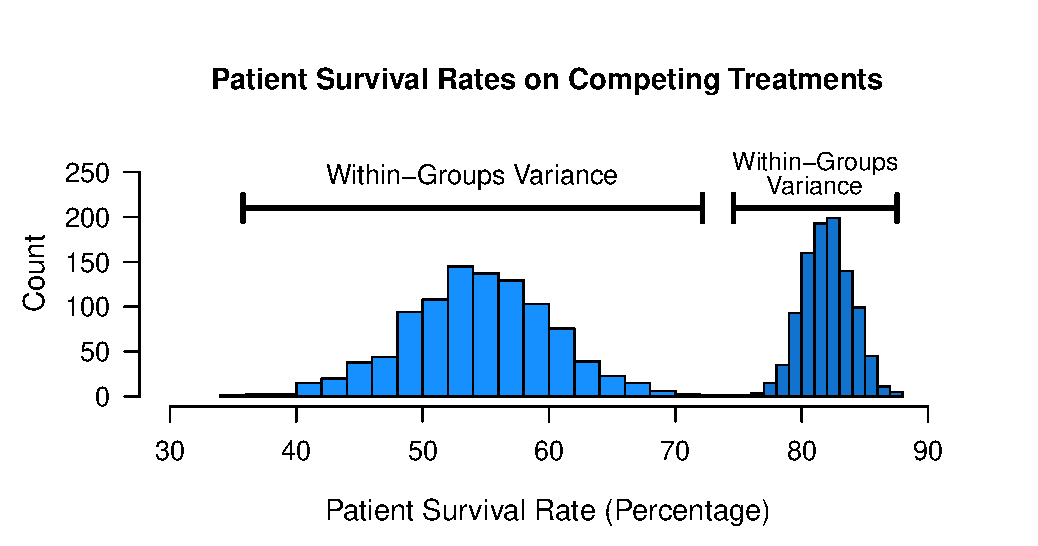
\includegraphics[width=35pc]{anova03}
\label{fig:anova03}
\caption{Patient survival rates using two competing treatment regimens. Here, within-groups variance is illustrated, showing the spread of the measurements within each treatment group.}
\end{figure}

Likewise, in Figure \ref{fig:anova03}, we see the variance within groups. The treatment group in light blue has a larger variance than does the treatment group on the right in dark blue. Unlike between-groups variance, here we rather see smaller within-group variances. The reason for this is that a larger within-groups variance means that we need an even \textbf{bigger} between-groups variance to compensate (or a much larger sample size): this type of variance obscures the effect of our treatment by introducing additional noise to our model.

Formally, we define these measurements as sums of squares, calculated:
\begin{eqnarray*}
SS_{residual} &=& \sum_{i=1}^n \left(y_i - \hat{y}_i\right)^2 \\
SS_{treatment} &=& \sum_{i=1}^n \left(\hat{y}_i-\bar{y}_i\right) \\
SS_{total} &=& SS_{residual}+SS_{treatment} \\
\end{eqnarray*}

\subsection{The \textit{F}-Test}

The \textit{F}-test is used to take these observed variances and give a standardized test statistic allowing us to quantify the magnitude of the difference observed between our treatment groups. It is calculated by:
\begin{equation}
F = \frac{MS_{treatment}}{MS_{residual}}
\end{equation}

The mean square ($MS$) statistics are calculated by:
\begin{equation*}
F = \frac{\text{Between-groups}}{\text{Within-groups}} = \frac{MS_{treatment}}{MS_{residual}} = \frac{SS_{treatment}/(I-1)}{SS_{residual}/(n-1)}
\end{equation*}
where $I$ is the number of treatments and $n$ is the total number of observations.

Values of the \textit{F}-statistic above 1 indicate that the observed results are further and further inconsistent with the null hypothesis. However, the exact value of $F$ needed for statistical significance will vary as a function of your degrees of freedom.

\subsection{Follow-Up Analyses}

\subsubsection{Post-Hoc Tests}

\subsubsection{Planned Comparisons and Linear Contrasts}

\section{Cautions and Considerations}

\subsection{Assumptions}

This test assumes that:

\begin{enumerate}
\item the samples are normally-distributed;
\item the samples are independent;
\item the cases represent a simple random sample of the population; and
\item the variances of the treatment groups are equal.
\end{enumerate}

\subsection{Robustness of the Test}

\section{Implementation in R}

\subsection{aov() vs. lme() vs. lmer()}

\section{Case Study: [STUDY]}

\section{Exercises}

\section{Additional Resources}


	%!TEX root=../book.tex

\chapter{Multifactor Studies}

\section{Overview of Multiple ANOVAs}

\section{Cautions and Considerations}

\section{Implementation in R}

\section{Case Study: [STUDY]}

\section{Exercises}

\section{Additional Resources}

	%!TEX root=../book.tex

\chapter{Multifactor Studies with Replication}

	
	\part{Describing Relationships and Predicting Values}
	%!TEX root=../book.tex

\chapter{Correlation}

\section{Overview of Correlation}

\subsection{Scatterplots}
Okay, so this is something that we could have presented back a few chapters ago when we talked about data visualization. Unfortunately, that wouldn't have worked with the example we were using, so instead of completely switching gears on you, we decided to wait until now to present it.

Scatterplots are used to display data using cartesian coordinates. For instance, we may wish to visualize the growth of the U.S. population by decade (Figure \ref{fig:correlation01}).

\begin{figure}[h]
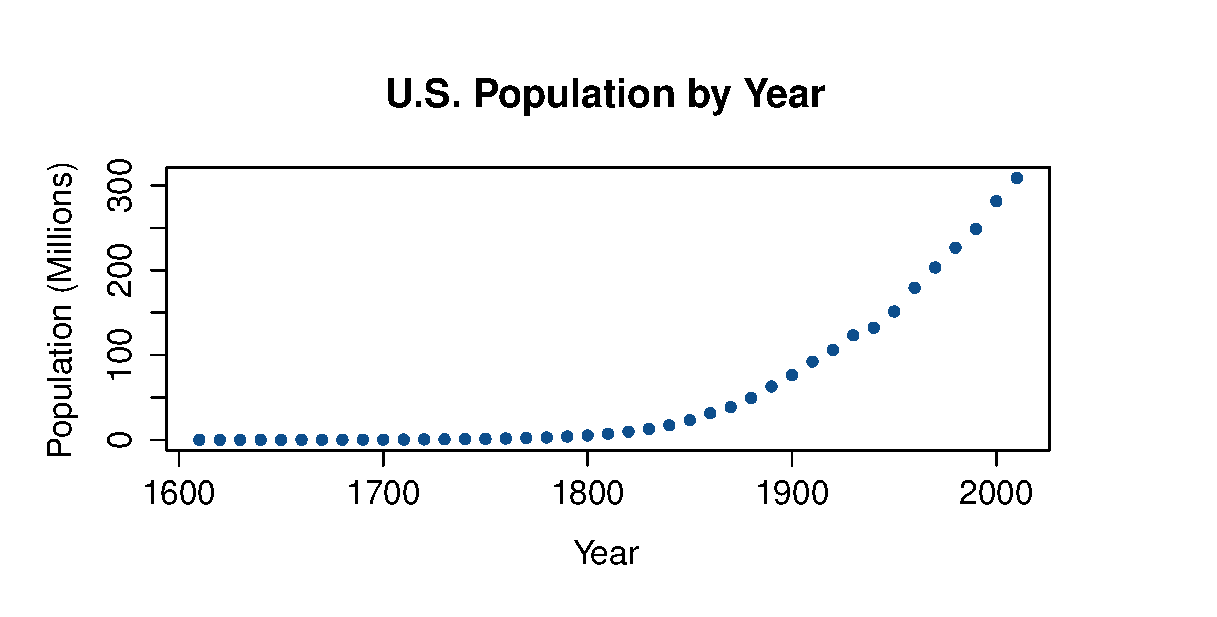
\includegraphics[width=35pc]{correlation01}
\label{fig:correlation01}
\caption{United States population by decade: 1600 through 2010}
\end{figure}

\subsubsection{Scatterplots with Categorical Variables}
Additionally, we can use scatterplots to visualize data with categorical indicators. For example, if we were interested in the depression and anxiety scores of patients with mild, moderate, and severe bipolar diagnoses (Figure \ref{fig:correlation02}).

\begin{figure}[h]
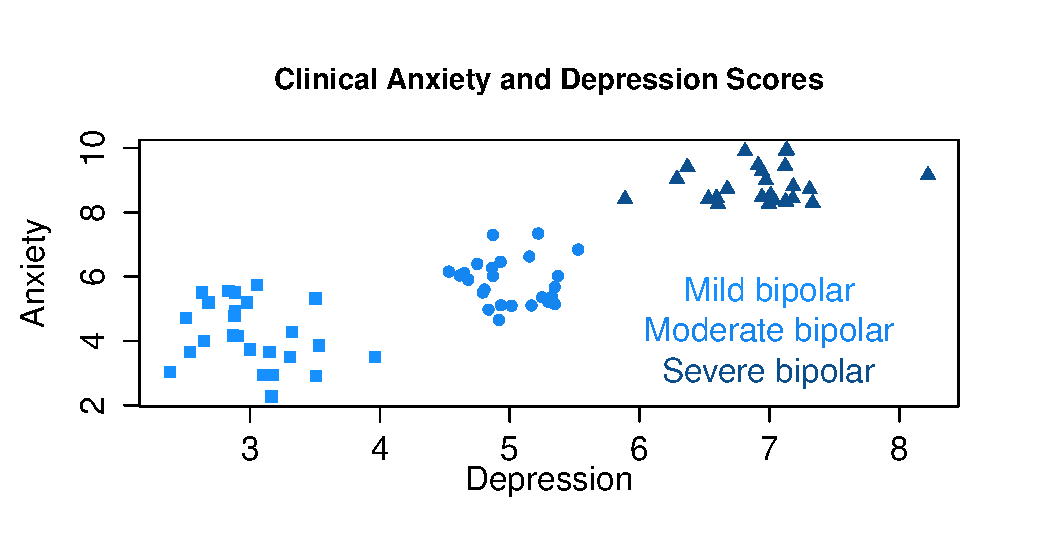
\includegraphics[width=35pc]{correlation02}
\label{fig:correlation02}
\caption{Depression and anxiety scores of patients with bipolar depression}
\end{figure}

\subsection{Correlation: Measuring Linear Association}
Woah, hold up now: measuring linear association? This sounds like we're heading towards some scary waters. Linear association? I thought this wasn't supposed to be a mathy book!

Don't worry, we didn't lie to you. That's just a bit of a scary term for a not-so-scary concept. \textbf{Linear association}, in its most basic form, just means that when you increase one variable by so many units, another variable increases by so many other units. For instance, let's say that for every degree Fahrenheit we increase, we increase the number of daily neighborhood ice cream sales by 10 cones. That's easy, right?

And that's all that correlation is measuring: the degree to which a change in one variable coincides with a change in another variable. Now, importantly, this doesn't mean that one causes the other. As a matter of fact, that's so important that it gets its own section a little ways down the page. But, as long as we keep that in the back of our minds for now, we can go ahead and define correlation as:

\begin{eqnarray}
\rho_{X,Y} =& \frac{\text{cov}(X,Y)}{\sigma_X\sigma_Y} &\text{ for a population} \\
r=& \frac{1}{n-1}\sum_{i=1}^n\left(\frac{x_i-\bar{x}}{s_x}\right)\left(\frac{y_i-\bar{y}}{s_y}\right) &\text{ for a sample}
\end{eqnarray}

So, although this looks like we're going back into the Forbidden Forest, it's a pretty straightforward couple of equations: they're saying that this correlation coefficient \(r\) is just equal to the covariance of two variables, \(x\) and \(y\), divided by the product of their standard deviations. Or, put another way, it's the amount that two variables change together divided by the amount of that change that we can attribute to chance.

This will then give us a single value, \(r\), which can be anywhere from -1 to +1. Now, in this case, both negative and positive 1 mean the same thing (or pretty close to the same thing): this coefficient tells us about the strength of the relationship between the two variables. So, if we have \(r=-1\), that means that for every increase of \(x\) units of one variable, we decrease by \(y\) units of a second variable. Likewise, for \(r=1\), this tells us that for every \(x\) units that we increase one variable, we increase the other by exactly \(y\) units. Finally, if we have \(r=0\), that tells us that there is absolutely no relationship between our two variables. In other words, you could increase one variable by over 9000 units and absolutely nothing would change in your second variable.

Unfortunately, most of us will never see a correlation that strong in real life: that would mean that there is absolutely no variance of your data. Now, if we're talking about a physical law and measuring it with incredibly high-precision instruments, it's entirely possible that we will have a correlation that strong. However, in most studies, there will be some random variance thrown in that weakens the correlation.

So remember:

\begin{eqnarray*}
r=& \pm1 &\implies \text{strong correlation} \\
r=& 0 &\implies \text{weak correlation}
\end{eqnarray*}


\subsection{Correlation Matrices and Multiple Correlation}
We know that correlation is a measure of dependence between two variables. However, there may be times when you want to examine multiple variables at once. In cases like this, it may be useful to create a \textbf{correlation matrix}. This is simply a lower-triangular matrix of correlations among multiple variables.

For instance, let's say that we want to see how adiposity in different parts of the body correlate. We may do something like:

\begin{framed}
\begin{Verbatim}[samepage=TRUE]
as.dist(cor(bodyFat))

          Neck    Chest   Abdomen  Hip
        +-------------------------------
  Chest | 0.766 
Abdomen | 0.728   0.911
    Hip | 0.705   0.823   0.860  
  Thigh | 0.668   0.708   0.736    0.881
\end{Verbatim}
\end{framed}

Here we can see the correlations between Neck, Chest, Abdomen, Hip, and Thigh adiposity---ranging from 0.67 to 0.91. However, what if we wanted to visualize these correlations as scatterplots? We might generate a lower-triangular scatterplot matrix using the \verb|pairs()| function (Figure \ref{fig:correlation03}):

\begin{framed}
\begin{Verbatim}[samepage=TRUE]
pairs(~Neck+Chest+Abdomen+Hip+Thigh,
    data=bodyFat,upper.panel=NULL)
\end{Verbatim}
\end{framed}

\begin{figure}[h]
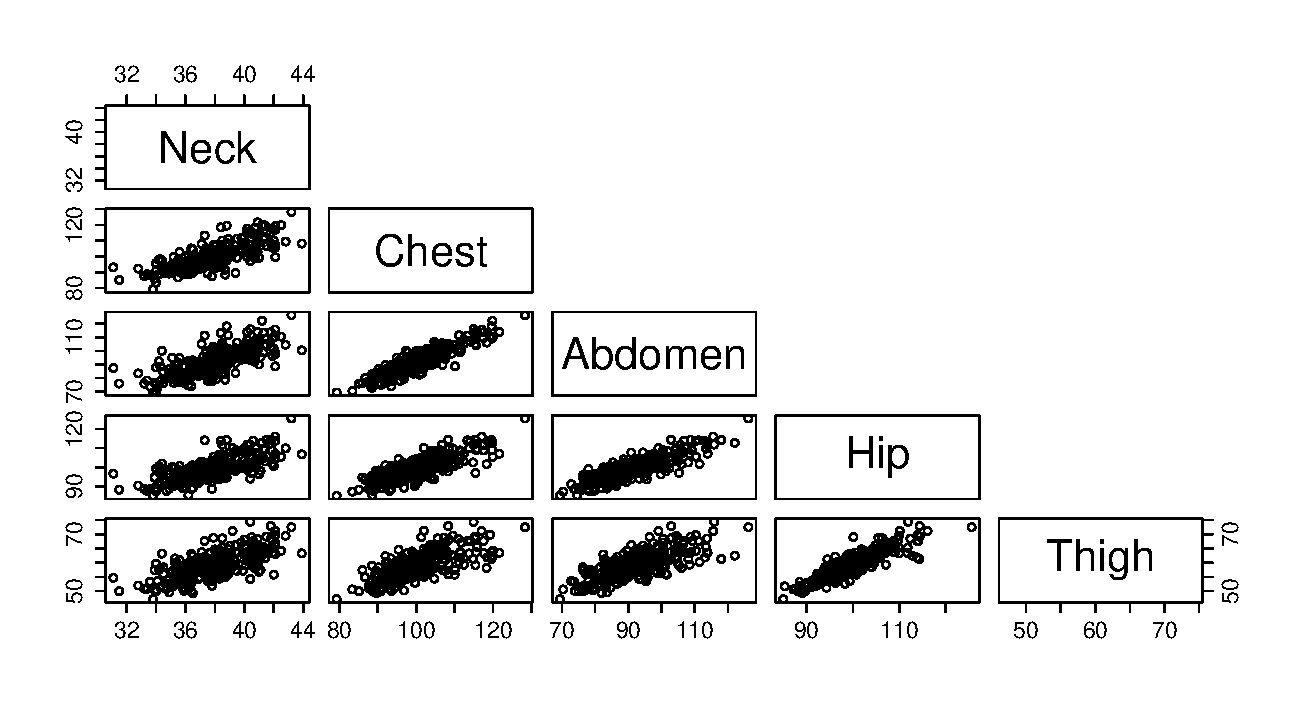
\includegraphics[width=35pc]{correlation03}
\label{fig:correlation03}
\caption{Lower-triangular scatterplot matrix for multiple correlations}
\end{figure}

Finally, we will likely want to assess the significance of these correlations. To do so, we will have to install the Hmisc package:

\begin{framed}
\begin{Verbatim}[samepage=TRUE]
install.packages("Hmisc")
library(Hmisc)
rcorr(as.matrix(bodyFat))
\end{Verbatim}
\end{framed}

This will return all bivariate correlations and levels of significance for the specified matrix. (NB: The data must be input as a matrix for this function to work. If you are using a data frame, first pass it through the \verb|as.matrix()| function.)

\subsection{Partial Correlations}
In our previous section, we looked at correlations among multiple variables. These were all referred to as \textbf{bivariate correlations} because each correlation only looked at exactly two variables. However, we saw that each of those 5 variables correlated significantly with each of the others. So it may be more appropriate to conduct a \textbf{partial correlation}: this will take two variables---say, Neck and Chest---and measure their degree of association after controlling for the effect of Abdomen, Hip, and Thigh. This approach is generally preferred if there are other known sources of covariance that you also measured.

\section{Cautions and Considerations}
\subsection{Causal Inferences}
Importantly, one cannot make causal inferences from correlational designs: if you think back to the chapter on research design, for a causal inference to by justified, there must be (1) temporal precedence; (2) covariation; and (3) nonspuriousness. Here, we violate the first and third assumptions. Regarding temporal precedence, neither of the measures that we are looking at clearly precedes the other: the measurements could be made simultaneously; one could always occur before the other; or the order of occurrence could be random at each point of measurement. Additionally, correlational studies don't have any control or experimental conditions in place to ensure that potential confounding variables are controlled for and don't give rise to spurious correlations.

Given these concerns, we are only able to say that Variable A and Variable B tend to covary: that is, when one changes in a certain way, the other is likely to change in a certain way. For instance, consider height and weight. Let's say that there is a positive correlation between the two (i.e., that taller people tend to weigh more and that people who weigh less tend to be shorter). We can say that someone who is 6'1" is likely to weigh more than someone who is 4'10"; however, it becomes silly to say that if someone loses weight, he or she will start shrinking in height. Likewise, by gaining weight, no one will ever grow taller. There is a general trend of the data; however, this does not mean that a change in one ever causes a change in the other.

\subsection{Linearity of the Relationship}
Another consideration when looking at correlations is the relationship between the two variables of interest. Namely, there must be a linear trend. In this context, a linear trend is going to mean that every time Variable A changes by \( x \) units, Variable B will change by \(y\) units. For instance, take the four plots in Figure \ref{fig:correlation04}.

\begin{figure}[h]
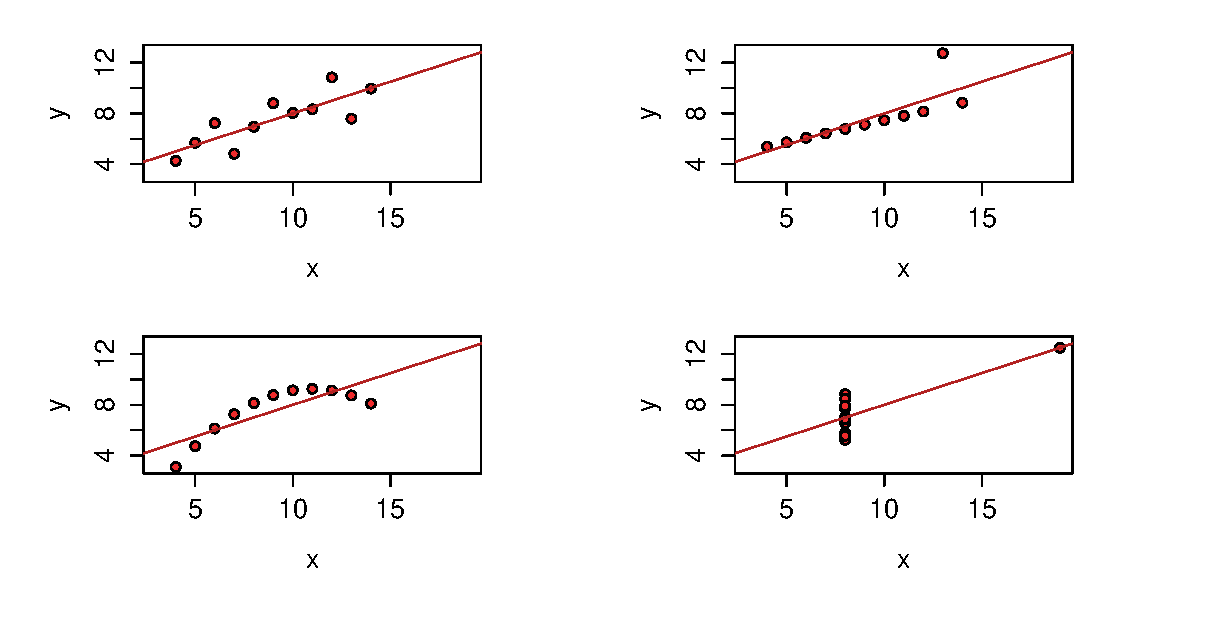
\includegraphics[width=35pc]{correlation04}
\label{fig:correlation04}
\caption{Four separate data sets, each with the same mean and correlation. Source: \href{http://en.wikipedia.org/wiki/Correlation}{Wikipedia}}
\end{figure}

Here we have four different relationships between our two variables with the same regression line plotted against all of them. As far as a correlation is concerned, the data follow that solid line.

\subsection{Sensitivity to the Distribution}
Also important is the distribution of the data. Although the degree of dependence between two variables $X$ and $Y$ is unaffected by transformations of the data where both $X$ and $Y$ are transformed by constants, the strength of correlation is highly impacted by the range of values sampled. Generally, the wider the range that is sampled, the stronger the correlation will be between the two measures.

Take, for instance, Figure \ref{fig:correlation06}. In orange are the unrestricted data, giving a correlation of $r=0.897$. Yet, when we restrict our range to only values of $X$ on the interval $(0,1)$, that correlation drops to $r=0.387$ although no transformations or other alterations were made to the data. Given these concerns, there have been attempts to correct for this range restriction; however we will not detail them here. Generally, this is not often a major issue to researchers; however, if you know that your data will be somehow restricted, it is good to keep in mind that this may impact the correlation coefficient.

\begin{figure}[h]
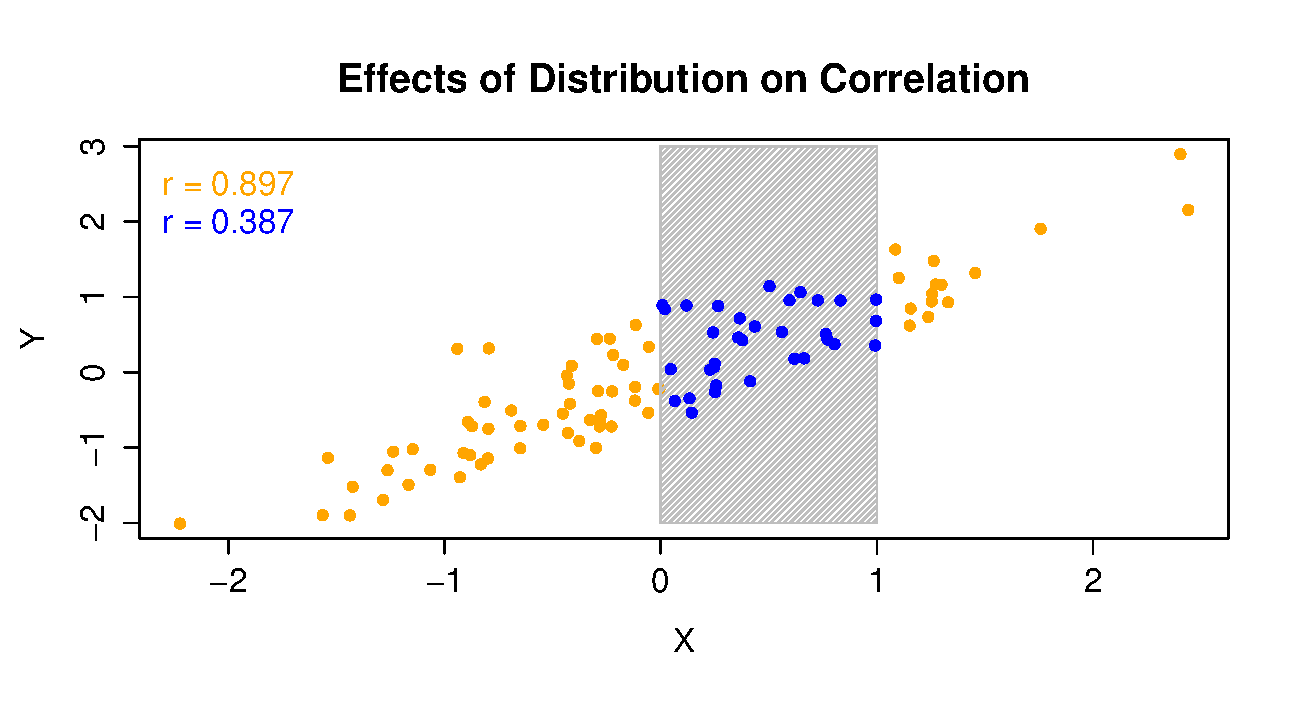
\includegraphics[width=35pc]{correlation06}
\caption{Pearson correlation coefficients between X and Y are shown when the two variables' ranges are unrestricted (orange) and when the range of X is restricted to the interval (0,1) (blue)}
\label{fig:correlation06}
\end{figure}

\section{Implementation in R}

\subsection{Correlation}
Using R, if we want to look at the correlation between two variables, we can do so using the \verb|cor()| function. Alternately, if we want to see if there is a \textbf{significant} correlation between those two variables, we use the \verb|cor.test()| function. For instance, if we wished to see the correlation between amounts of neck and chest fat, we would run:

\begin{framed}
\begin{Verbatim}[samepage=TRUE]
cor.test(bodyFat$Neck, bodyFat$Chest)

	Pearson's product-moment correlation

data:  bodyFat$Neck and bodyFat$Chest
t = 18.7782, df = 247, p-value < 2.2e-16
alternative hypothesis: true correlation is not equal to 0
95 percent confidence interval:
 0.7102541 0.8136117
sample estimates:
      cor 
0.7668596 
\end{Verbatim}
\end{framed}

As we can see, there was a correlation between the two variables of $r=0.77$ and this reached a level of statistical significance, $t = 18.78$; $p\text{-value}<0.001$. Because our $p$-value was below the $0.05$ threshold, we can conclude that the relationship between the two variables actually exists. This means that individuals with more neck fat tend to also have more chest fat, and vice versa.

\subsection{Partial Correlation}

To run a partial correlation in R, we will execute something like:

\begin{framed}
\begin{Verbatim}[samepage=TRUE]
source("http://www.yilab.gatech.edu/pcor.R")

neck <- bodyFat$Neck
chest <- bodyFat$Chest
others <- subset(bodyFat, select=c(Abdomen:Thigh))

pcor.test(neck,chest,others)

   estimate  p.value  statistic
  0.344  9.7e-09   5.73  249
\end{Verbatim}
\end{framed}

We can see that the observed correlation drops from \(r=0.766\) with the bivariate correlation to \(r=0.344\) with the partial correlation. This means that, when we control for the effects of Abdomen, Hip, and Thigh adiposity, neck and chest still covary significantly with a correlation of about 0.34.

\section{Case Study: National Education Trends}

These data are taken from the Census' American Community Survey. Here, we have two columns that we're interested in: \verb|highSchoolorHigher| and \verb|perCapitaIncome|. We would like to see if there is a relation between a state's per capita income and the proportion of its residents to have completed high school or higher. So let's start by constructing a scatterplot of the two variables, seen in Figure \ref{fig:correlation05}:

\begin{figure}[h!]
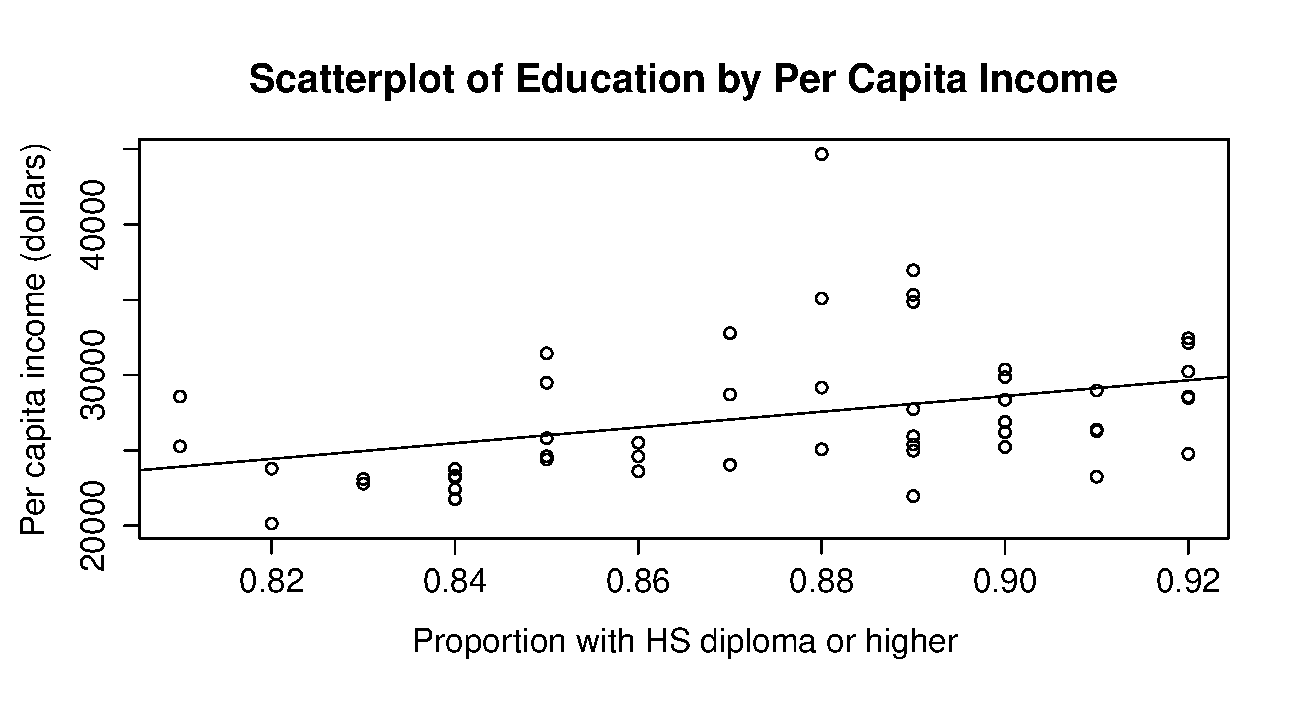
\includegraphics[width=35pc]{correlation05}
\label{fig:correlation05}
\caption{Scatterplot of perCapitaIncome and HighSchoolOrHigher}
\end{figure}

As we can see, there appears to be a positive linear relationship between per capita income and the proportion of a state's residents having a high school diploma or higher. Our next step is then to quantify the strength of this relationship. To do this, we will perform a bivariate correlation, giving us the results:

\begin{framed}
\begin{Verbatim}[samepage=TRUE]
  Pearson's product-moment correlation

data:  perCapitaIncome and HighSchoolOrHigher
t = 2.7752, df = 49, p-value = 0.007788
alternative hypothesis: true correlation is not equal to 0

95 percent confidence interval:
 0.1034750 --- 0.5847427

sample estimates:
      cor 
0.3685491 
\end{Verbatim}
\end{framed}

As we can see, there are several noteworthy items presented in this table. Firstly, we have a \textit{t}-statistic of 2.78. This is above the 1.96 threshold that we set, indicating that our correlation is probably going to be significant. From there, we can look at our \textit{p}-value (0.008) and see that it is below the 0.05 threshold, indicating that we do indeed have a significant correlation.

If it weren't obvious from the scatterplot above, this is a positive correlation with a Pearson's $r=0.37$, meaning that there exists a fair positive relationship between our two variables. I.e., when one is larger, the other will also tend to be larger.

\section{Exercises}

\prob Download the \href{https://raw.githubusercontent.com/faulconbridge/appliedStats/master/LaTeX/part03/data/correlationEx01.csv}{Patient Satisfaction data set} from GitHub. This dataset contains information from patients surveyed at various hospitals following their treatment to assess their satisfaction with the experience. We will be using these data for the following exercises.
\prob Do patient ratings for \verb|nursesCommunicateWell| and \verb|doctorsCommunicateWell| correlate with one another? Provide evidence to back up your answer. Include a scatterplot of the data.
\prob Now perform a partial correlation between those two same variables, but controlling for\\\verb|givenInformationAboutRecovery| and \verb|staffExplainedMedications|.
\prob Create a lower-diagonal correlation matrix correlating all of the variables included in the dataset (except for the hospital ID). What correlations are significant? Are there any that are non-significant? (NOTE: You will have to remove null values using the \verb|na.omit()| function for this to work properly.
\prob Construct a scatterplot matrix of all bivariate correlations using the code:
\begin{framed}
\begin{Verbatim}[samepage=TRUE]
pairs(~nursesCommunicateWell + doctorsCommunicateWell +
  receivedImmediateHelp + painManagedByTreatment +
  staffExplainedMedications + bathroomsAlwaysClean +
  givenInformationAboutRecovery + rateHospitalPositively,
  data=ex01, upper.panel=NULL)
\end{Verbatim}
\end{framed}
  
Do any of the scatterplots look concerning? Look for outliers, non-linear trends, etc.
\prob \textbf{Test yourself:} Choose two new variables and performa bivariate correlation test. Do they correlate significantly? Do you think there are any other variables that should be controlled for? If so, perform a partial correlation, controlling for those additional variables. Do the results differ? Explain why they do. Comment on the assumptions made by the correlation tests you have run. Are they met? Are any violated?
\prob Download the \href{https://raw.githubusercontent.com/faulconbridge/appliedStats/master/LaTeX/part03/data/correlationCaseStudy.csv}{Census American Community Survey} from GitHub. This dataset, used in the case study above, contains information about employment and other demographic characteristics nationwide.
\prob Is there a correlation between \verb|noHighSchoolDiploma| (the proportion of residents without a HS diploma or GED equivalent) and \verb|publicTransit| (the proportion of residents who use public transit to go to and from work)?
\prob Is there a correlation between \verb|HighSchoolOrHigher| and \verb|percentOnSNAP|? Justify your findings and include at least one figure.
\prob Is there a correlation between \verb|medianRent| and \verb|percentImpoverished|? Are there any variables we might want to control for using a partial correlation?
\prob \textbf{Test yourself:} Choose some (or all) of the variables in this dataset and make a correlation matrix for them. Choose a correlation that looks interesting or surprising and investigate it further. If applicable, perform a partial correlation test rather than a bivariate correlation.

\section{Additional Resources}

\begin{enumerate}
\item \href{https://github.com/faulconbridge/appliedStats/tree/master/LaTeX/part03/data}{All data sets} used in the chapter
\item \href{https://github.com/faulconbridge/appliedStats/tree/master/LaTeX/part03/RScripts}{All R scripts} used in the chapter
\item \href{https://github.com/faulconbridge/appliedStats/blob/master/LaTeX/part03/answers/correlation.md}{Answer key} to the chapter's exercises
\end{enumerate}
	%!TEX root=../book.tex

\chapter{Simple Linear Regression}

\section{Overview of Simple Linear Regression}

\subsection{Uses of Simple Linear Regression}
In the last chapter we touched briefly on the idea of using the value of one variable to predict the value of another. Where correlation is used to describe the magnitude of the relationship between two variables, a tool called \textbf{simple linear regression} takes that relationship and uses it to predict the values of Variable B, given some arbitrary value of Variable A. In this context, however, we refer to the \(x\) variable as our \textbf{explanatory variable} or our \textbf{regressor} and to the \(y\) variable as the \textbf{response variable}.

So, knowing that we use regression as a predictive tool, what \textit{is} it, exactly? Well, thankfully, it's a pretty straightforward thing that we can define as:

\begin{equation}
y = \beta_0 + \beta_1\cdot x
\label{eqn:regression01}
\end{equation}

So before we explain this equation, we need you to reach way back into those murky memories of your eighth grade math class when you were talking about the equation of a line. Remember that whole ``slope-intercept form'' lecture? Well, in case you don't, the equation of a line looks something like:
\begin{equation*}
\hat{y}=m\cdot x+b
\end{equation*}
where $m$ is the slope and $b$ is the intercept. Sound familiar?

Alright, now let's compare those two equations. Aside from using different variable names, they're identical to one another. All regression boils down to is drawing lines to connect a bunch of points on the page. And here you thought it was going to be scary!

Although regression is actually a bit more than drawing a line to connect the dots, the basic idea behind it is that for two variables there exists an equation with two basic constants---a slope and an intercept---that allows us to predict the value of $Y$ if we already know $X$.

But, although we know that equation exists, how do we figure it out? To do that we'll turn to something called \textbf{least squares estimators}.

\subsection{Least Squares Fitting}

If you think back to Equation \ref{eqn:regression01}, our two coefficients were $\beta_0$ and $\beta_1$. Those refer to the population coefficients: that is, if we were able to measure every single instance of $X$ and $Y$ in all of the universe, those would be the coefficients that we could derive from the population. In most cases, however, that isn't possible and so we use least squares estimates of $\beta_0$ and $\beta_1$ which we refer to as $\hat{\beta}_0$ and $\hat{\beta}_0$ (pronounced ``beta-null hat'' and ``beta-one hat'').

We can visualize this process in Figure \ref{fig:regression01}. Here, we see a number of data points as white circles. There is also a solid black line that represents a possible line of best fit. However, are the predicted data points (solid black circles) as close to the observed data as possible? Looking at the red dashed line between our predictions and observations, it looks like we could do a better job reducing that difference.

\begin{figure}[h]
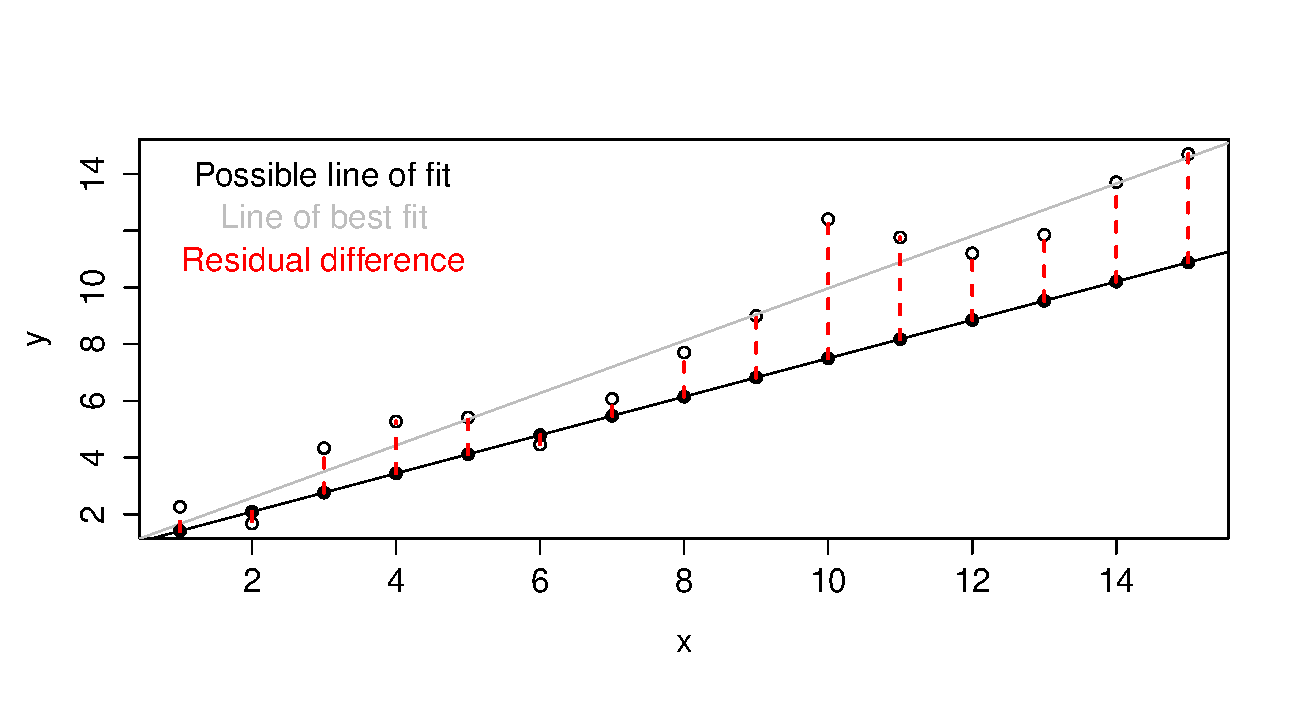
\includegraphics[width=35pc]{regression01}
\caption{Data with a least-squares line of best fit (grey), one potential line of best fit (black), and the residual difference between the predicted and observed values (red). Lease squares fitting seeks to minimize the overall distance between every observed value and predicted value, resulting in a single line of best fit.}
\label{fig:regression01}
\end{figure}

Minimizing that difference between our predicted and observed values is exactly what least squares estimation seeks to do. In fact, we can see the least squares line of best fit as the light grey line in Figure \ref{fig:regression01}. The residual difference in this line is mathematically as small as it possibly can be.

How we actually do this involves a bit of calculus so we aren't going to go into too much detail here. However, from that calculus we can derive these two estimates of our coefficients:
\begin{eqnarray*}
\hat{\beta}_1 &=& \frac{\sum_{i=1}^n\left(X_i-\bar{X}\right)\left(Y_i-\bar{Y}\right)}{\sum_{i=1}^n\left(X_i-\bar{X}\right)^2}\\
\hat{\beta}_0 &=& \bar{Y}-\hat{\beta}_1\cdot \bar{X}
\end{eqnarray*}

Thankfully, these aren't equations that you're liable to ever have to understand or use (unless you just really want to): least squares fitting is automated by every modern statistical package. Even your TI-84 calculator is happy to do it for you. The point, rather, is that given a set of data, there are these mathematical tools that we can use to attempt to model the relationship between our variables, even though this is mostly a behind-the-scenes operation.

\subsection{Coefficient of Determination}

The whole of a simple linear regression boils down to just a couple numbers, one of which is the \textbf{coefficient of determination}, denoted $R^2$ (pronounced ``R-squared''). This statistic represents the proportion of the variance seen in the data that is explained by the model.

If you think back to the chapter \textit{Measuring Uncertainty}, variance is the squared average distance of a data point from the mean. Let's take Figure \ref{fig:regression03} as an example. Here, we see that there is a regression equation fitted to the data with an $R^2=0.39$, indicating that about 39\% of the variance observed within the data is explained by the model.

\begin{figure}[h]
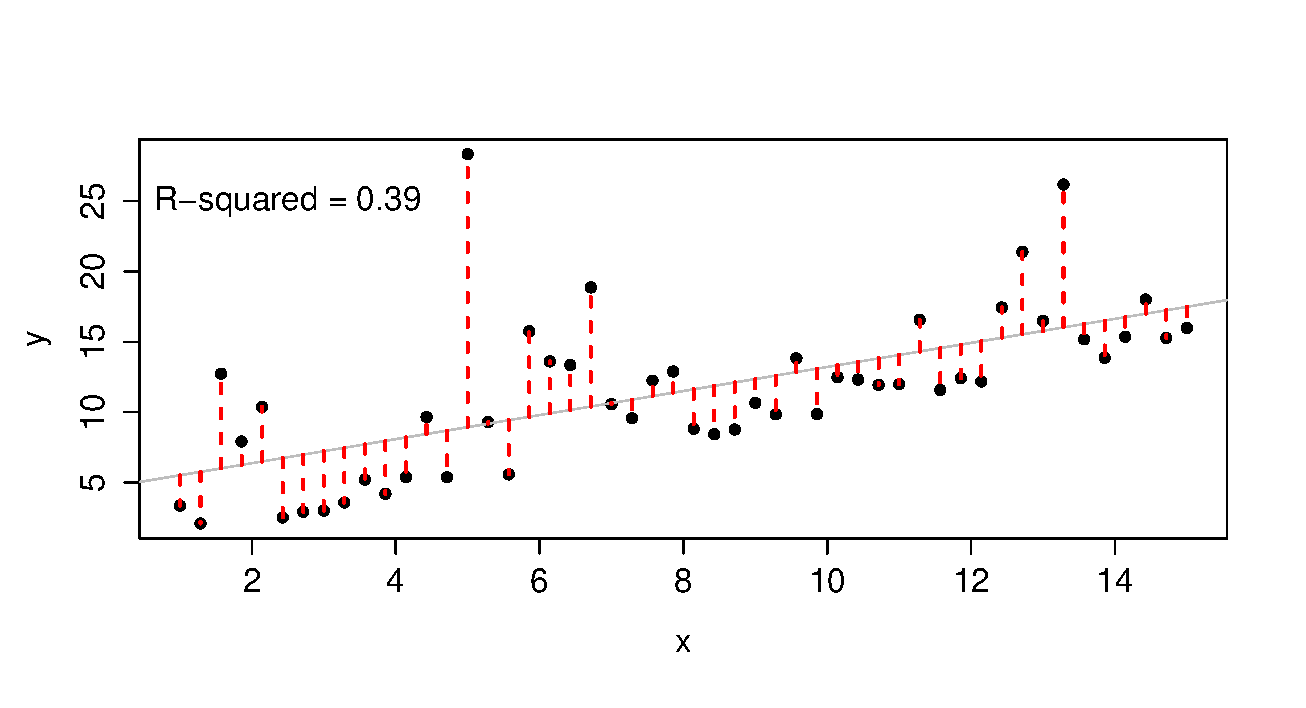
\includegraphics[width=35pc]{regression03}
\label{fig:regression03}
\caption{Regression model with approximately 39\% of the observed variance explained.}
\end{figure}

Now, it's important to recognize that the line of best fit that we've plotted doesn't describe our data perfectly. This is because there is an inherent bit of error---random variability---in any dataset (and thereby any equation that we use to model it). Given this, a better definition of Equation \ref{eqn:regression01} is:
\begin{equation}
\hat{y} = \beta_0 + \beta_1\cdot x+\epsilon
\label{eqn:regression02}
\end{equation}
where $\epsilon$ represents that error. In our example, we can see that each point does not vary above or below the regression line by an equivalent amount: if there were no error, then the distance of all of the points from the regression line, above and below, should sum out to 0. (That is, points above the line are equally far from it as are points below the line.)

The equation that we use to model our data will never be able to perfectly explain all of that random variation which is why we use the $R^2$ statistic to quantify the proportion of it that \textbf{can be} explained. Correspondingly, a larger value of $R^2$ corresponds to a model that better fits the data.

As with Pearson's $r$ in correlational designs, $R^2$ varies from 0 to 1. (Note: Pearson's $r$ can fall on the interval (-1, 1); however, because the coefficient of determination is squared, it can only fall on the interval (0, 1). Any negative number multiplied by another negative number will always equal a positive number.)

\subsection{Residuals}

The formal calculation of the proportion of the variance that is explained by the model is a bit more complicated than what we presented above. To understand how $R^2$ is calculated, we first need to understand the concept of \textbf{residuals}. A residual is defined as the difference between an observed and predicted value. If we look back to Figure \ref{fig:regression03}, the residuals are represented by the dashed red lines. This is equivalent to the error term ($\epsilon$) that we mentioned in the previous section.

When calculation $R^2$, we use the formula:
\begin{equation}
R^2 \equiv 1-\frac{SS_{residual}}{SS_{total}}
\end{equation}
where $SS_{residual}$ is the residual sum of squares and $SS_{total}$ is the total sum of squares. To get an idea of what these two terms mean, let's look at Figure \ref{fig:regression04}. On the left we see a representation of the total sum of squares for four data points. This is derived by finding the squared distance between each observed data point and the arithmetic mean of $y$ and adding them all together. Mathematically, we represent this as:
\begin{equation*}
SS_{total} =\sum_i \left(y_i-\bar{y}\right)^2
\end{equation*}
The idea here is that we want to find out the total distance of our data from their mean: a larger value means that the data are farther dispersed from their mean; a smaller value indicates that they all cluster closer to their mean value. (Likewise, a value closer to 0 indicates a weaker relationship between the two variables: it shows that $y$ is unaffected by the value of $x$.)

Next we have the residual sum of squares. This value represents the sum of the squared distances of each point from its predicted value. In other words, it's a measure of how accurately the data can be fitted to a line. Mathematically, we represent this as:
\begin{equation*}
SS_\text{residual}=\sum_i \left(y_i - \hat{y}_i\right)^2
\end{equation*}
As with our total sum of squares, a higher value for our residual sum of squares indicates a larger discrepancy between our predicted and observed values of $y$ whereas a smaller value indicates a better fit of the model to the data. By then comparing the ration of these two values, we can assess what proportion of the total variance our model is able to explain, and thus how good of a fit it provides.

\begin{figure}[h]
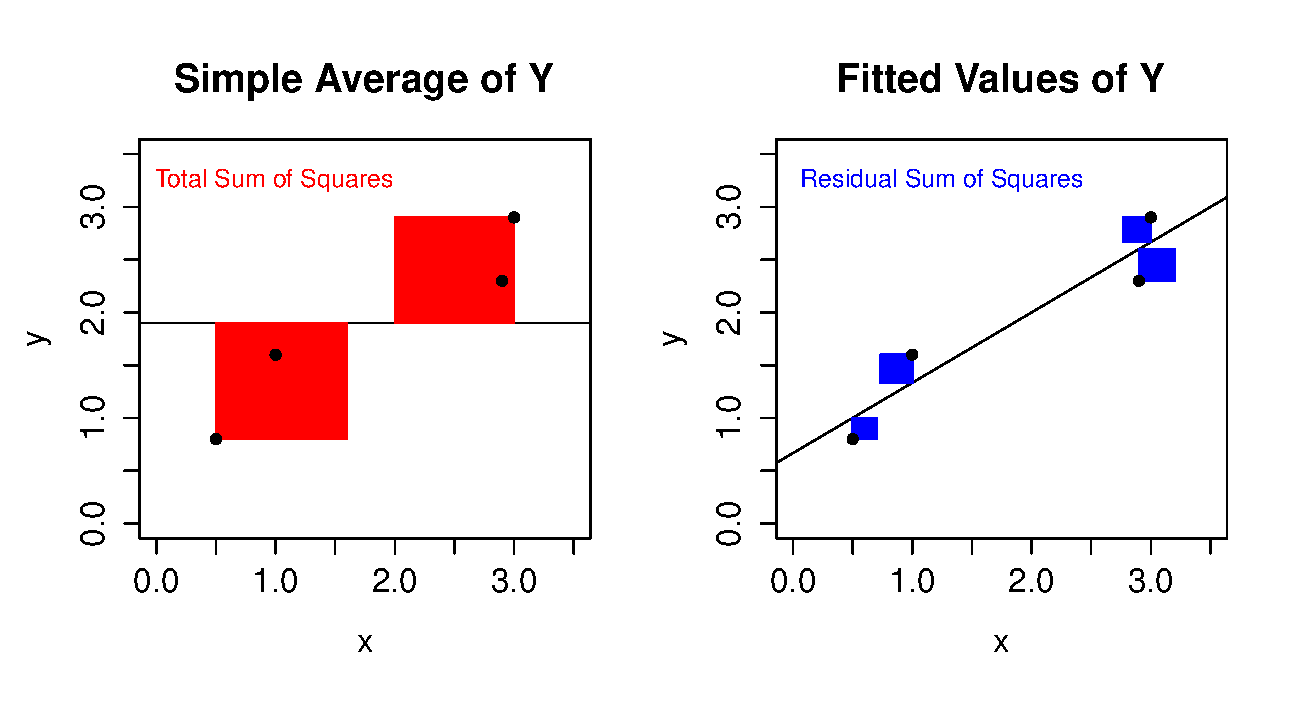
\includegraphics[width=35pc]{regression04}
\label{fig:regression04}
\caption{$R^2$ is defined generally as $1-\frac{SS_{residual}}{SS_{total}}$. Here, we see the total sum of squares (red) as the sum of the squared distance from each observation to the arithmetic mean of $y$ ($\bar{y}$). The residual sum of squares (blue) is computed as the sum of the squared distance from each observation to its predicted value.}
\end{figure}

\section{Cautions and Considerations}


\subsection{Basic Assumptions}

page 182

\subsection{Outliers and Influential Points}


\section{Case Study: [STUDY]}

\begin{figure}[h]
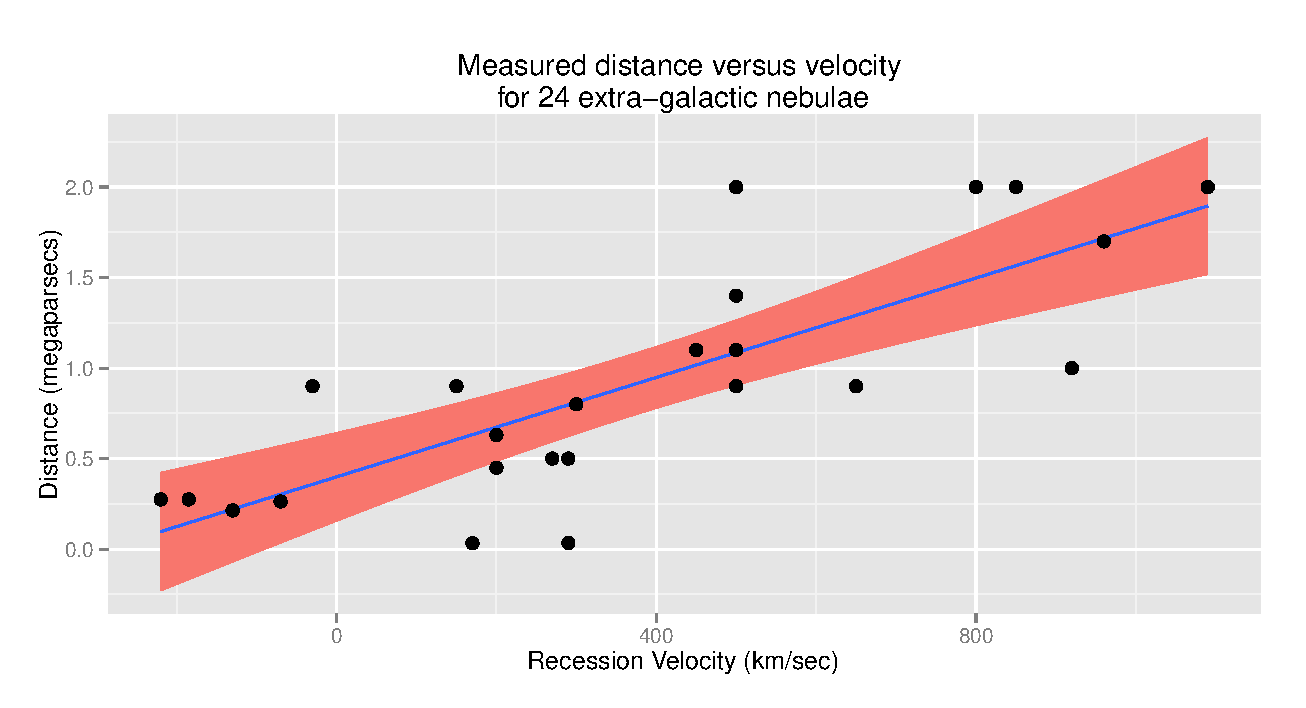
\includegraphics[width=35pc]{regression02}
\label{fig:regression02}
\caption{Measured distance versus velocity for 24 extra-galactic nebulae. Data from Hubble, E. (1929). \href{http://www.ncbi.nlm.nih.gov/pmc/articles/PMC522427/}{A relation between distance and radial velocity among extra-galactic nebulae.} \textit{Proceedings of the National Academy of Sciences of the United States of America, 15}, 168-173. Line of best fit plotted in blue with a 95\% confidence interval for the regression line in red.}
\end{figure}
\section{Exercises}


\section{Additional resources}
	%!TEX root=../book.tex

\chapter{Multiple Regression}

	%!TEX root=../book.tex

\chapter{Logistic Regression}

\section{Overview of Logistic Regression}

\section{Cautions and Considerations}

\section{Implementation in R}

\section{Case Study: [STUDY]}

\section{Exercises}

\section{Additional Resources}

	%!TEX root=../book.tex

\chapter{Model Refinement and\\ Variable Selection}

	
	\part{Inferences from Unusual Data Structures}
	%!TEX root=../book.tex

\chapter{Time-Series Data and Serial Correlation}

\section{Overview of Time-Series Tools}

\section{Cautions and Considerations}

\section{Implementation in R}

\section{Case Study: [STUDY]}

\section{Exercises}

\section{Additional Resources}

	%!TEX root=../book.tex

\chapter{Factor Analysis and\\ Principle Component Analysis}

	%!TEX root=../book.tex

\chapter{Rank-Ordered Data}

	%!TEX root=../book.tex

\chapter{Tables of Counts,\\ Proportions, and Odds}

\section{Overview of Chi-Squared Tests}

\section{Cautions and Considerations}

\section{Implementation in R}

\section{Case Study: [STUDY]}

\section{Exercises}

\section{Additional Resources}

	
	\part{Supplemental Materials}
	%!TEX root=../book.tex

\chapter{Choosing the Right Analysis:\\ A Cheat Sheet}

	%!TEX root=../book.tex

\chapter{Getting Outside Help:\\ How to Share Data}


%%%%%%%%%%%%%%%%%%%
% End Matter
%%%%%%%%%%%%%%%%%%%

	% \appendix
	
	% \bibliographystyle{apacite}  % Reference style
	% \bibliography{}                     % References filename


%%%%%%%%%%%%%%%%%%%
% INDEX
%%%%%%%%%%%%%%%%%%%

	\printindex

%%%%%%%%%%%%%%%%%%%
% End document
%%%%%%%%%%%%%%%%%%%

	\end{document}